\documentclass{ctexart}
\usepackage{EC}
\begin{document}
\section{氧及其化合物}
\subsection{单质氧}
我们所熟知的氧的单质是氧气和臭氧.
\subsubsection{\ce{O2}}
\begin{substance}[\ce{O2}]
    氧气是无色气体,常压下在$90.2\K$时液化为淡蓝色的液体,在$54.4\K$时凝固为淡蓝色固体.\\
    氧气微溶于水,在室温常压下的溶解度大约为$10\text{ mg/L}$.
\end{substance}
\paragraph{\ce{O2}的结构}
\ce{O2}是少数几种具有偶数个电子而(在基态下)保持顺磁性的分子.基态\ce{O2}的分子轨道表示式为
\[KK\left(\sigma_{2\text{s}}\right)^2\left(\sigma_{2\text{s}}^\ast\right)^2\left(\sigma_{2\text{p}}\right)^2\left(\pi_{2\text{p}}\right)^4\left(\pi_{2\text{p}}^\ast\right)^2\]
需要注意的是,\ce{O2}尽管是特殊的,但它并没有发生s-p混杂.
\paragraph{\ce{O2}的制备}
制备氧气主要通过含氧化合物的分解\footnote{虽然更经济的方法是直接购买氧气罐.在工业上,通过液化的方法分离空气中的各组分已经是一项成熟的技术.}.实验室一般采取如下方法:
\begin{enumerate}[label=\tbf{\arabic*},topsep=0pt,parsep=0pt,itemsep=0pt,partopsep=0pt]
    \item 热分解\ce{KClO3}.分解的反应方程式为
        \begin{center}
            \ce{2KClO3(s) ->T[$\Delta$] 2KCl(s) + 3O2(g)}
        \end{center}
        这一反应需要$400\sim500\tccentigrade$的温度.如果加入\ce{MnO2}作为催化剂,则温度可以降低到$150\tccentigrade$,但产物中会不可避免地出现少量\ce{ClO2}.
    \item 热分解\ce{KMnO4}.分解的反应方程式为
        \begin{center}
            \ce{2KMnO4(s) ->T[$\Delta$] K2MnO4(s) + MnO2(s) + O2(g)}
        \end{center}
        如果所用的\ce{KMnO4}足够纯,那么这种办法可以生成非常纯净的\ce{O2}.
    \item 硝酸盐的热分解.以\ce{NaNO3}为例,分解的反应方程式为
        \begin{center}
            \ce{2NaNO3(s) ->T[$\Delta$] 2NaNO2(s) + O2(g)}
        \end{center}
    \item 过氧化物的分解.典型的有\ce{H2O2}在\ce{MnO2}催化下的分解
        \begin{center}
            \ce{2H2O2(aq) ->T[\ce{MnO2}] 2H2O(l) + O2(g)}
        \end{center}
        或者金属的过氧化物的热分解,如
        \begin{center}
            \ce{2BaO2(s) ->T[$\Delta$] 2BaO(s) + O2(g)}
        \end{center}
    \item 碱金属过氧化物与\ce{CO2}反应.\ce{Na2O2}与\ce{CO2}的反应以前被用于潜水员,消防员等的供氧设备中,而宇航密封舱则考虑到重量因素采用\ce{Li2O2}.反应的方程式如下:
        \begin{center}
            \ce{2M2O2 + 2CO2 -> 2M2CO3 + O2}\ \ \ $\left(\ce{M}=\ce{Li,Na}\right)$
        \end{center}
        这一反应的好处是既产生\ce{O2},又消耗\ce{CO2}.
\end{enumerate}
\paragraph{单线态\ce{O2}}
基态的\ce{O2}又称作\tbf{三线态氧},记作$^3\Sigma_g^-$.\\
\indent \ce{O2}的第一激发态又称作\tbf{单线态氧},其中两个电子成对地占据一个$\pi_{2\text{p}}^\ast$轨道,记作$^1\Delta_g$.\ce{O2}的第二激发态中,两个电子自旋反平行地分占$\pi_{2\text{p}}^\ast$轨道,记作$^1\Sigma_g^+$.\\
\indent 单线态\ce{O2}与基态\ce{O2}的能量差为$94.3\kJm$.由于单线态氧向基态的跃迁是自旋禁阻的,因此气相中的单线态氧的寿命较长,大约在$54\sim86\text{ ms}$左右.\\
\indent 单线态氧需要特殊的方法制备.
\begin{enumerate}[label=\tbf{\arabic*},topsep=0pt,parsep=0pt,itemsep=0pt,partopsep=0pt]
    \item 最简单的方法是\ce{H2O2}与\ce{NaOCl}的反应:
        \begin{center}
            \ce{H2O2(aq) + NaOCl(aq) -> NaCl(aq) + H2O(l) + O2($^1\Delta_g$,g)}
        \end{center}
        如果将\ce{Cl2}通入较浓的\ce{NaOH}与\ce{H2O2}的混合液中,可以看到闪烁的红光.这是由于单线态氧向基态跃迁所致.
    \item 在有机溶剂中,也可以采用亚磷酸酯和\ce{O3}在低温下形成加合物后分解的方式制备单线态\ce{O2}:
        \begin{center}
            \ce{P(OR)3 + O3 -> P(O3)(OR)3}\\
            \ce{P(O3)(OR)3 -> PO(OR)3 + O2($^1\Delta_g$)}
        \end{center}
\end{enumerate}

\indent 单线态氧在有机化学中有着重要的应用.作为烯烃的等电子体,它可以发生ene反应,环加成反应等周环反应.
\paragraph{固态\ce{O2}的结构}
固态\ce{O2}具有多种不同的晶型.
\begin{enumerate}[label=\tbf{\arabic*},topsep=0pt,parsep=0pt,itemsep=0pt,partopsep=0pt]
    \item $\alpha$-$\ce{O2}$\\
        \indent 浅蓝色晶体,属于单斜晶系,正常大气压下生成于$23.8\K$以下.
        \begin{figure}[H]
            \centering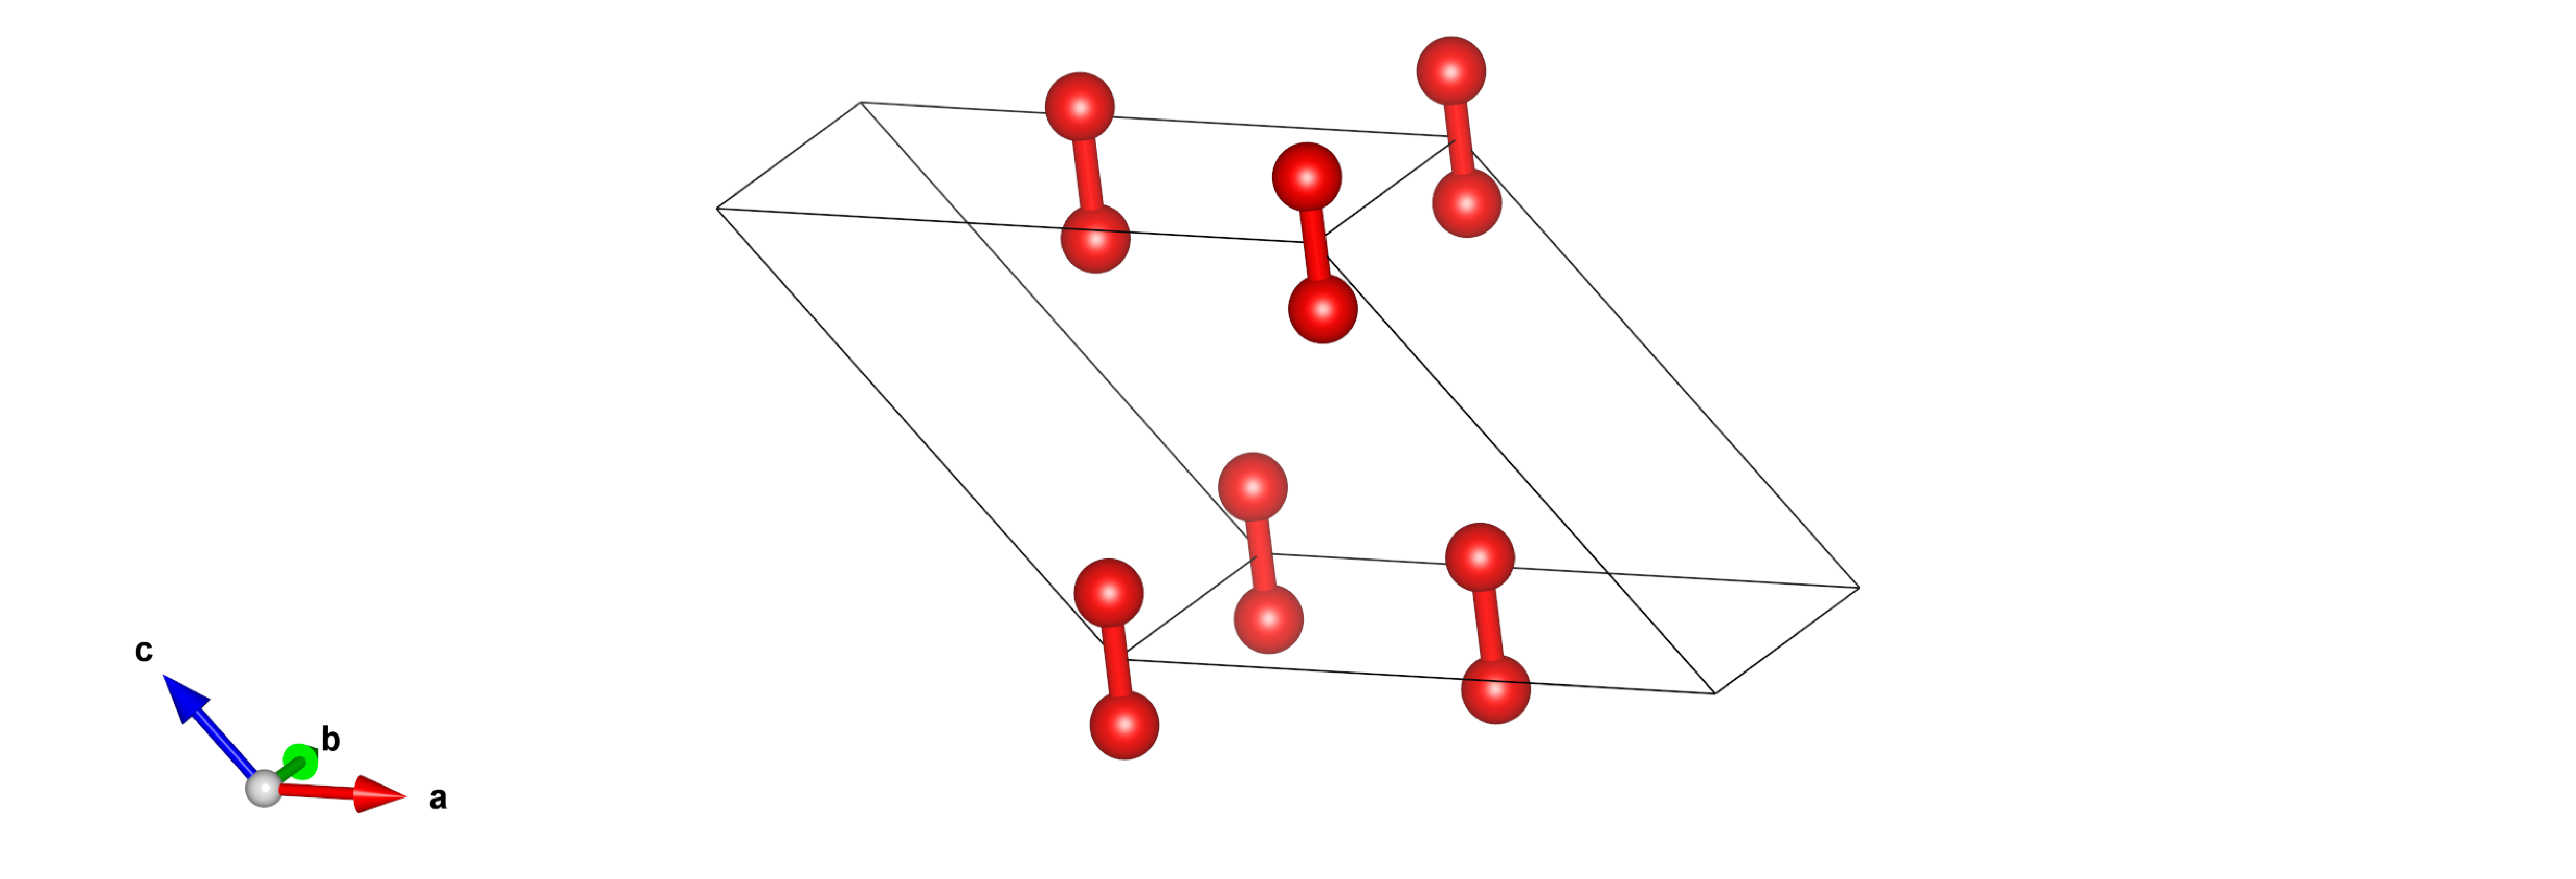
\includegraphics[scale=0.125]{picture/alpha-O2.eps}
            \caption{$\alpha$-$\ce{O2}$的晶体结构示意}
        \end{figure}
    \item $\beta$-$\ce{O2}$\\
        \indent 淡蓝色至粉红色晶体,属于三方晶系,正常大气压下生成于$43.8\K$以下.
        \begin{figure}[H]
            \centering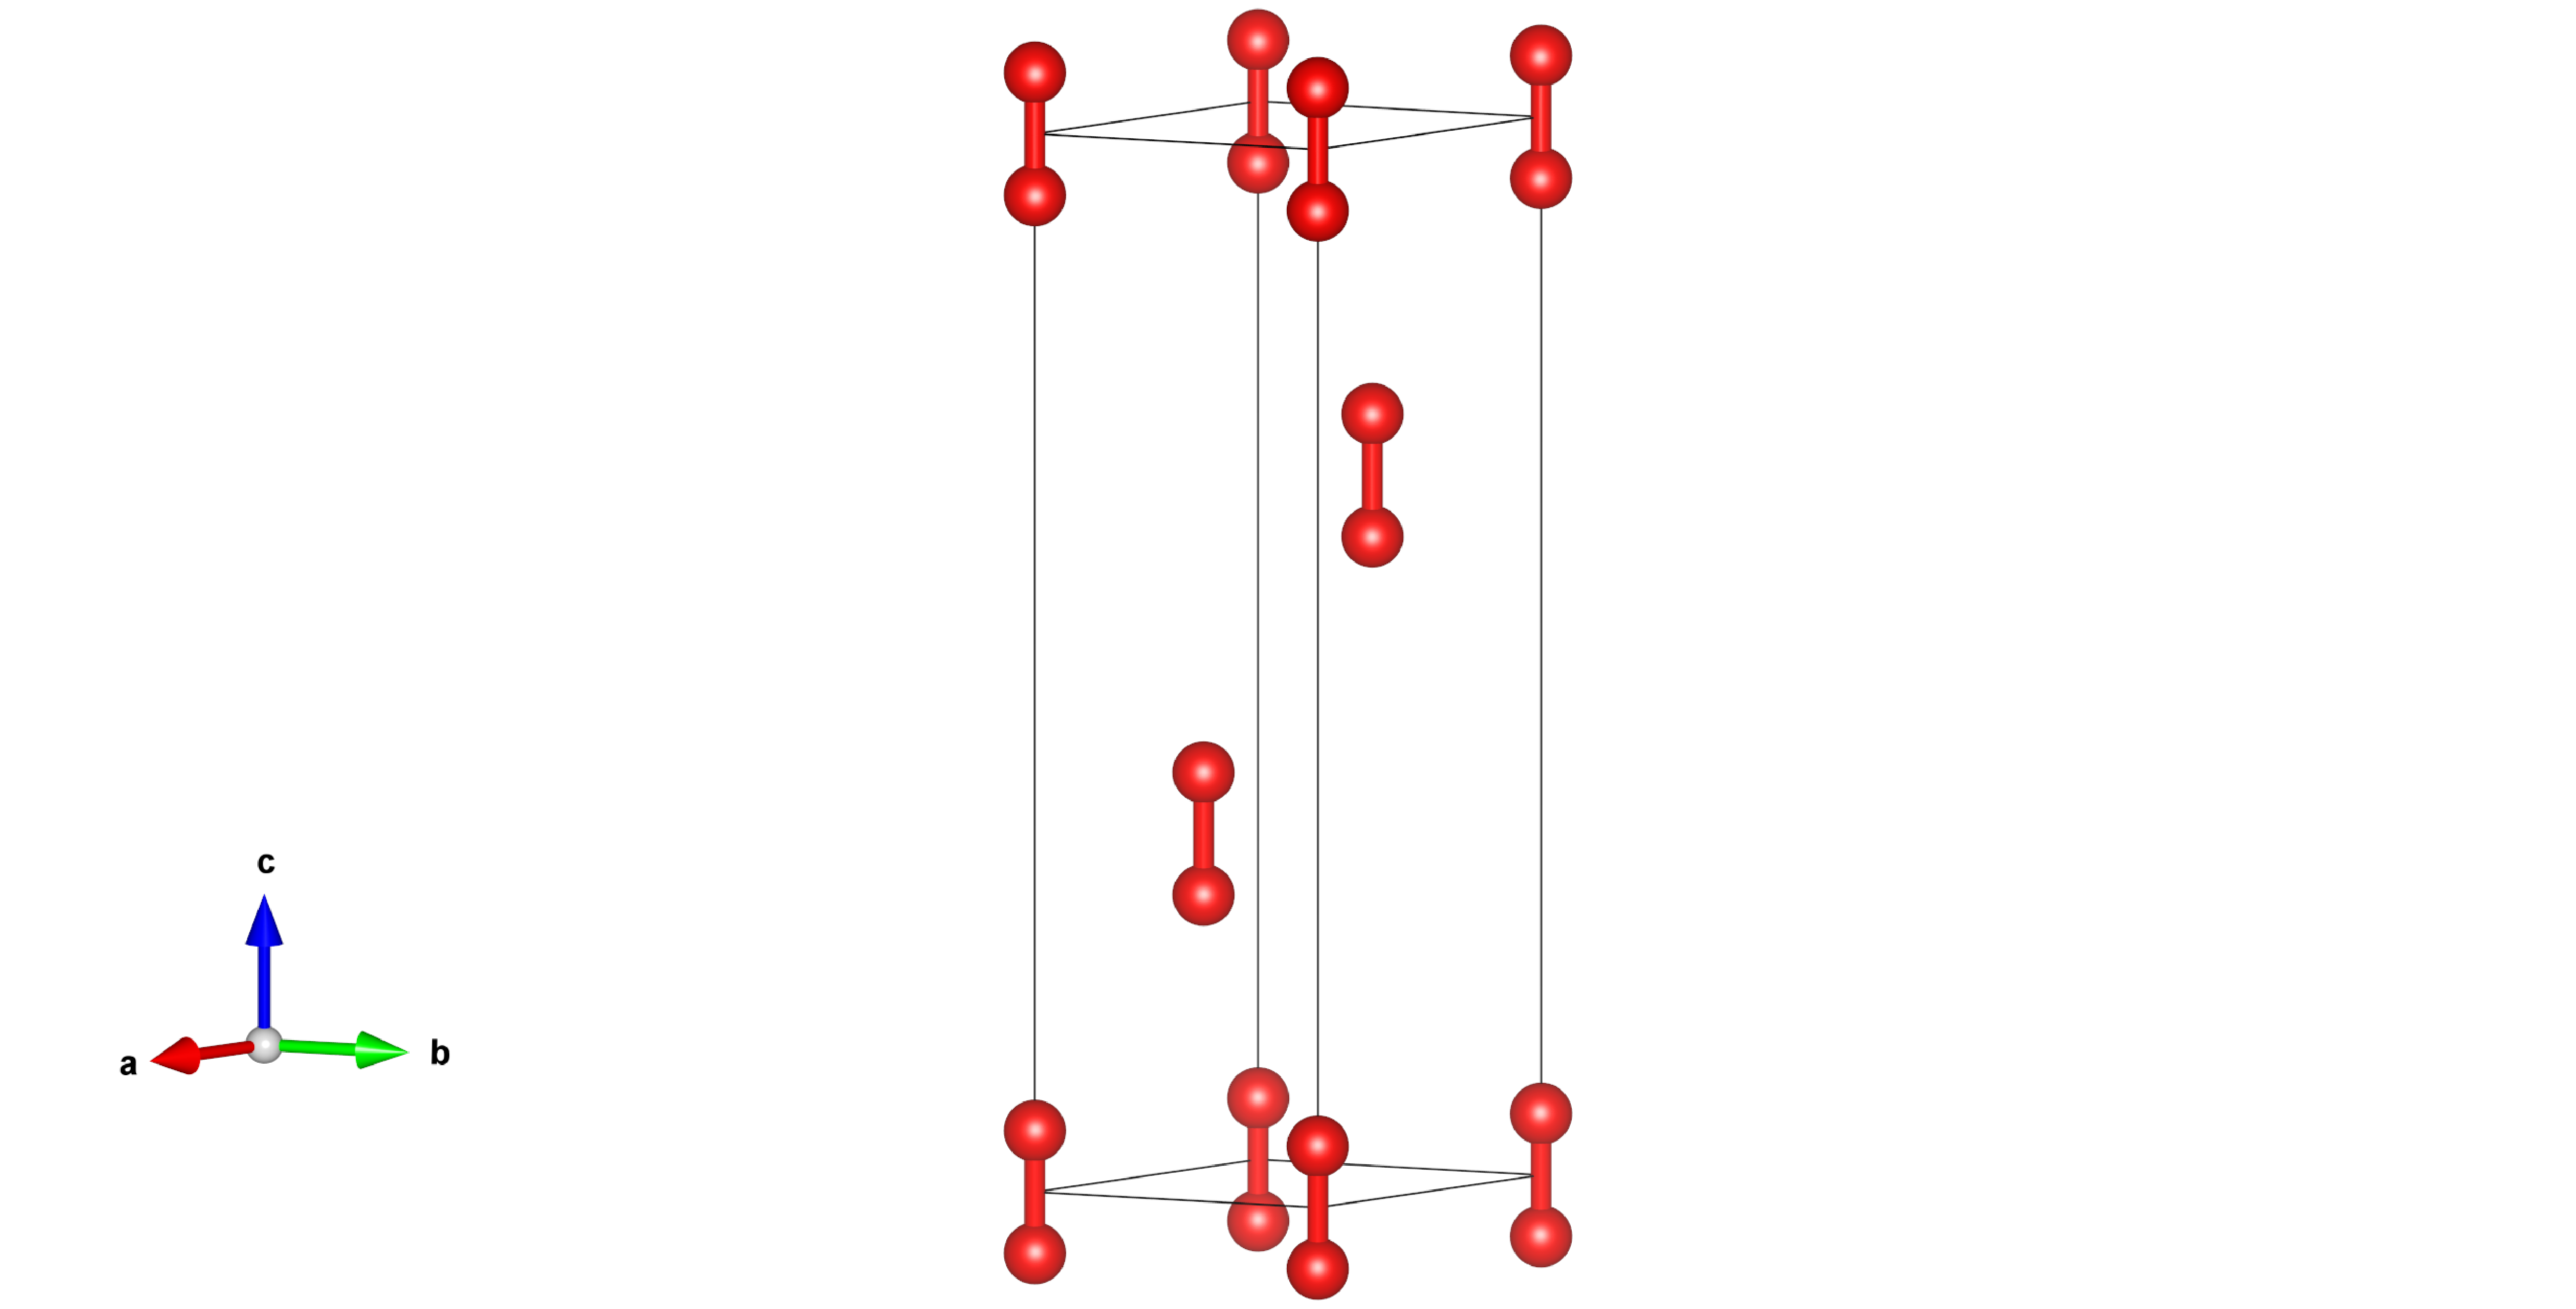
\includegraphics[scale=0.125]{picture/beta-O2.eps}
            \caption{$\beta$-$\ce{O2}$的晶体结构示意}
        \end{figure}
    \item $\gamma$-$\ce{O2}$\\
        \indent 淡蓝色晶体,属于立方晶系,正常大气压下生成于$54.4\K$以下.
        \begin{figure}[H]
            \centering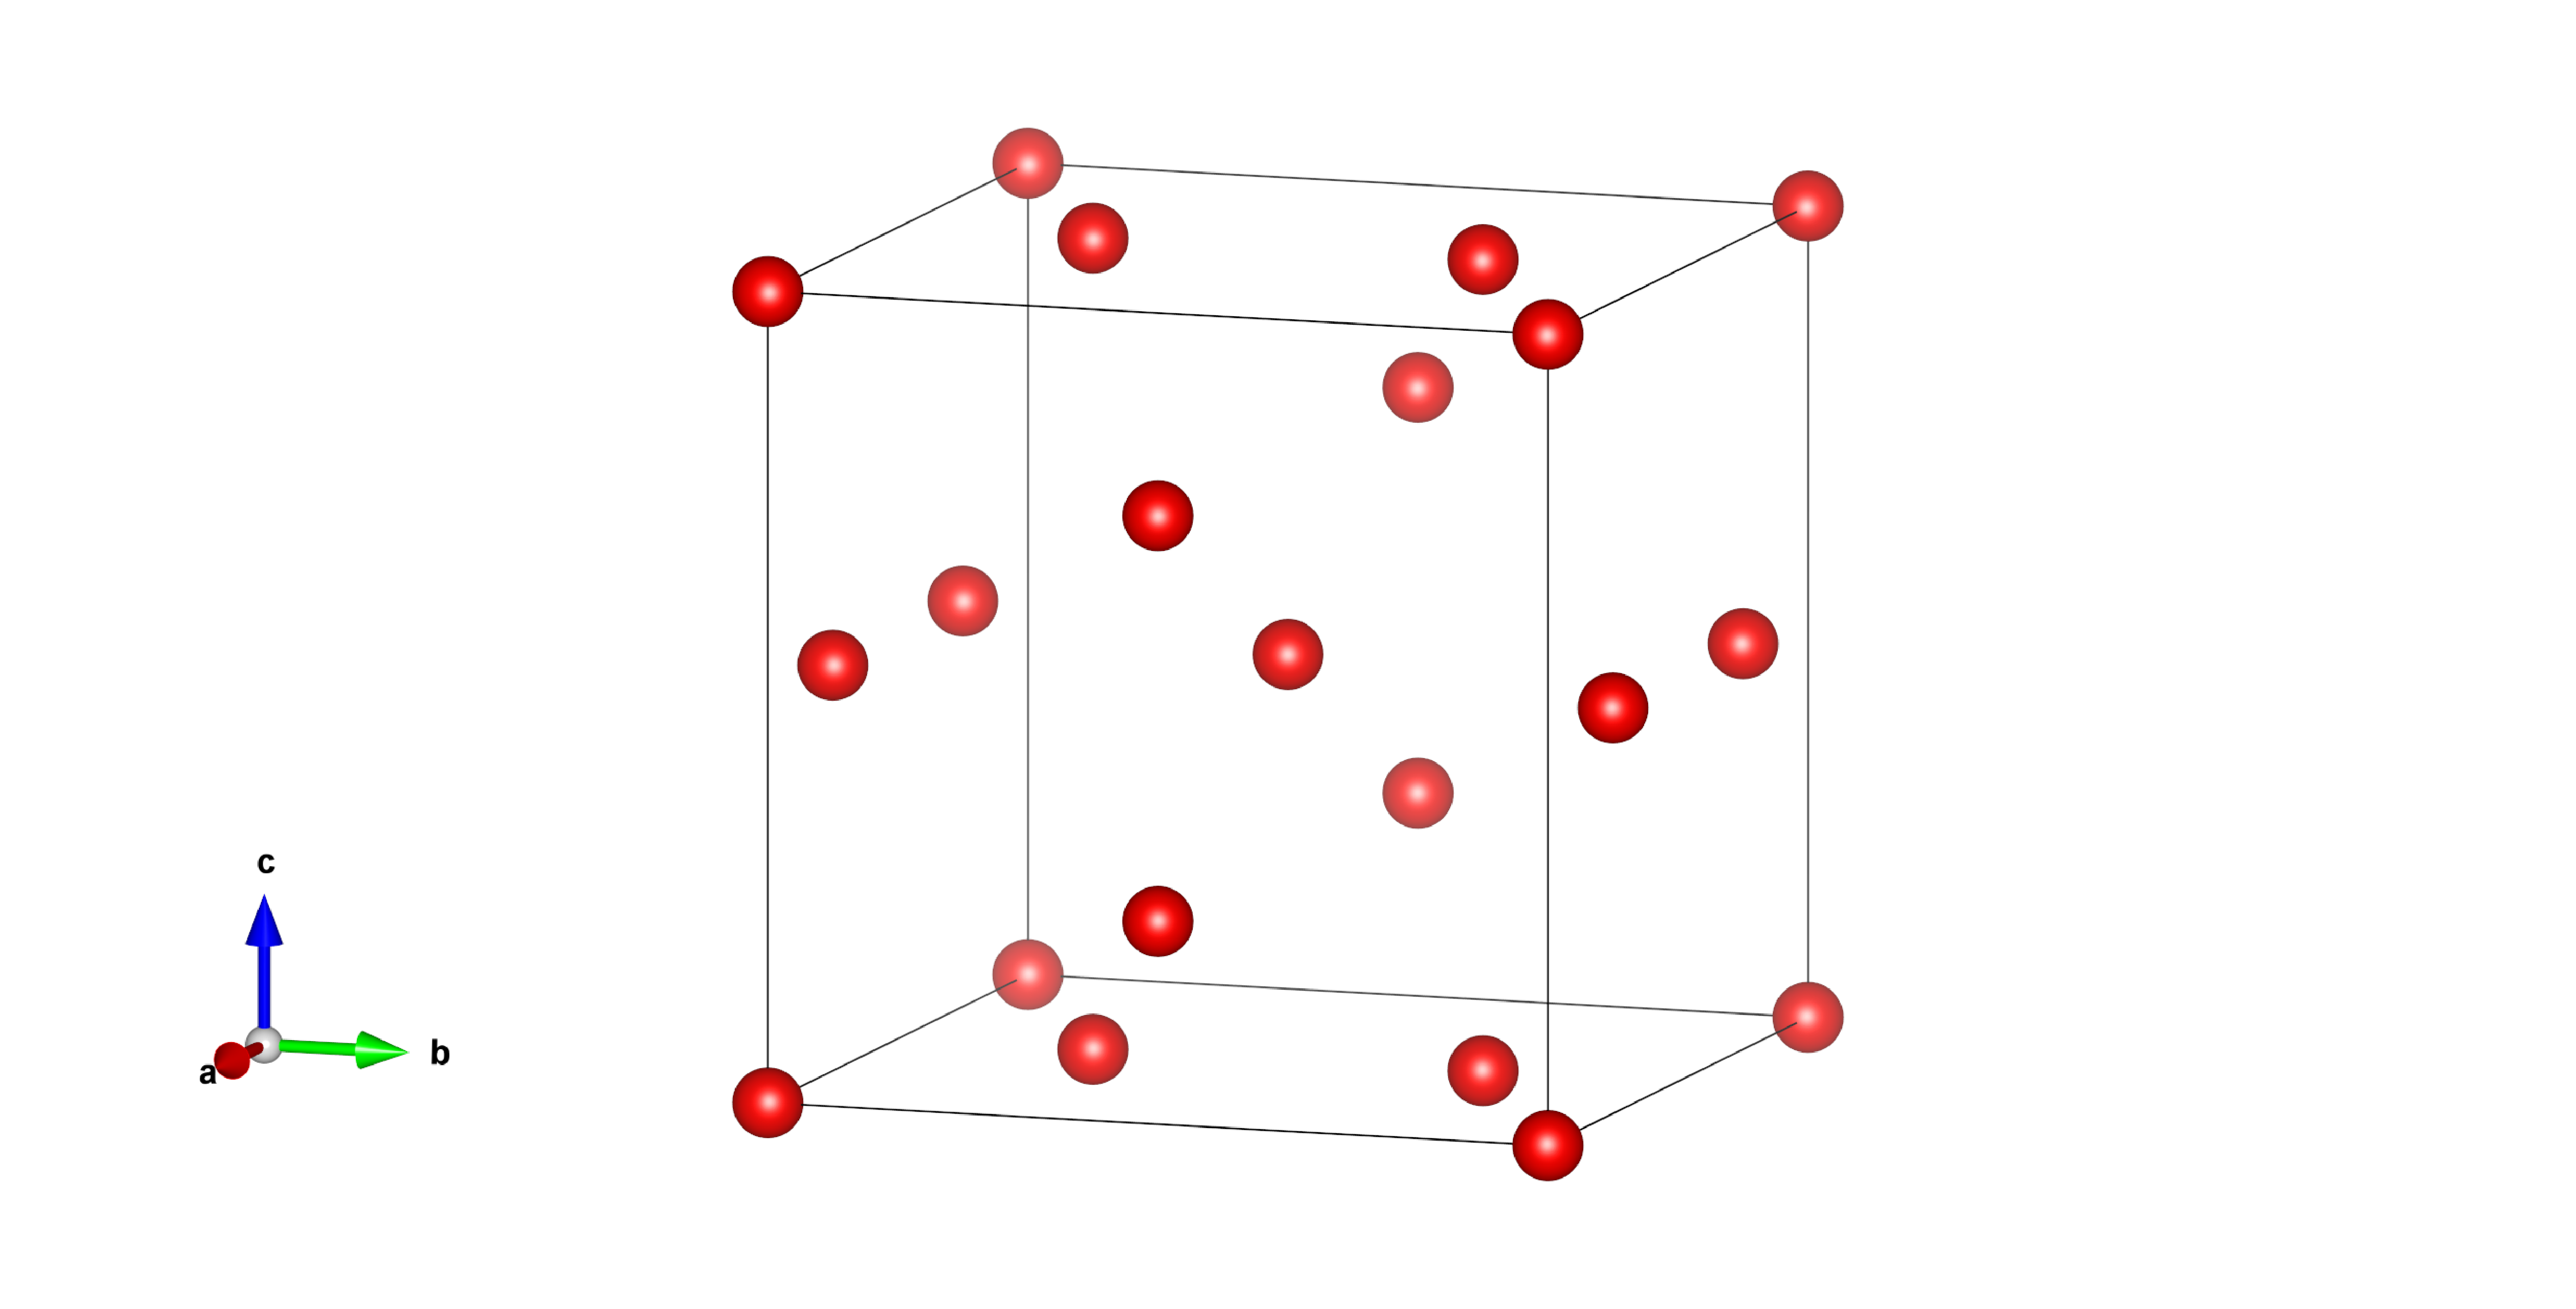
\includegraphics[scale=0.125]{picture/gamma-O2.eps}
            \caption{$\gamma$-$\ce{O2}$的晶体结构示意}
        \end{figure}
    \item $\delta$-$\ce{O2}$\\
        \indent 橙色晶体,属于正交晶系,室温时生成于$9\text{ GPa}$以上.
        \begin{figure}[H]
            \centering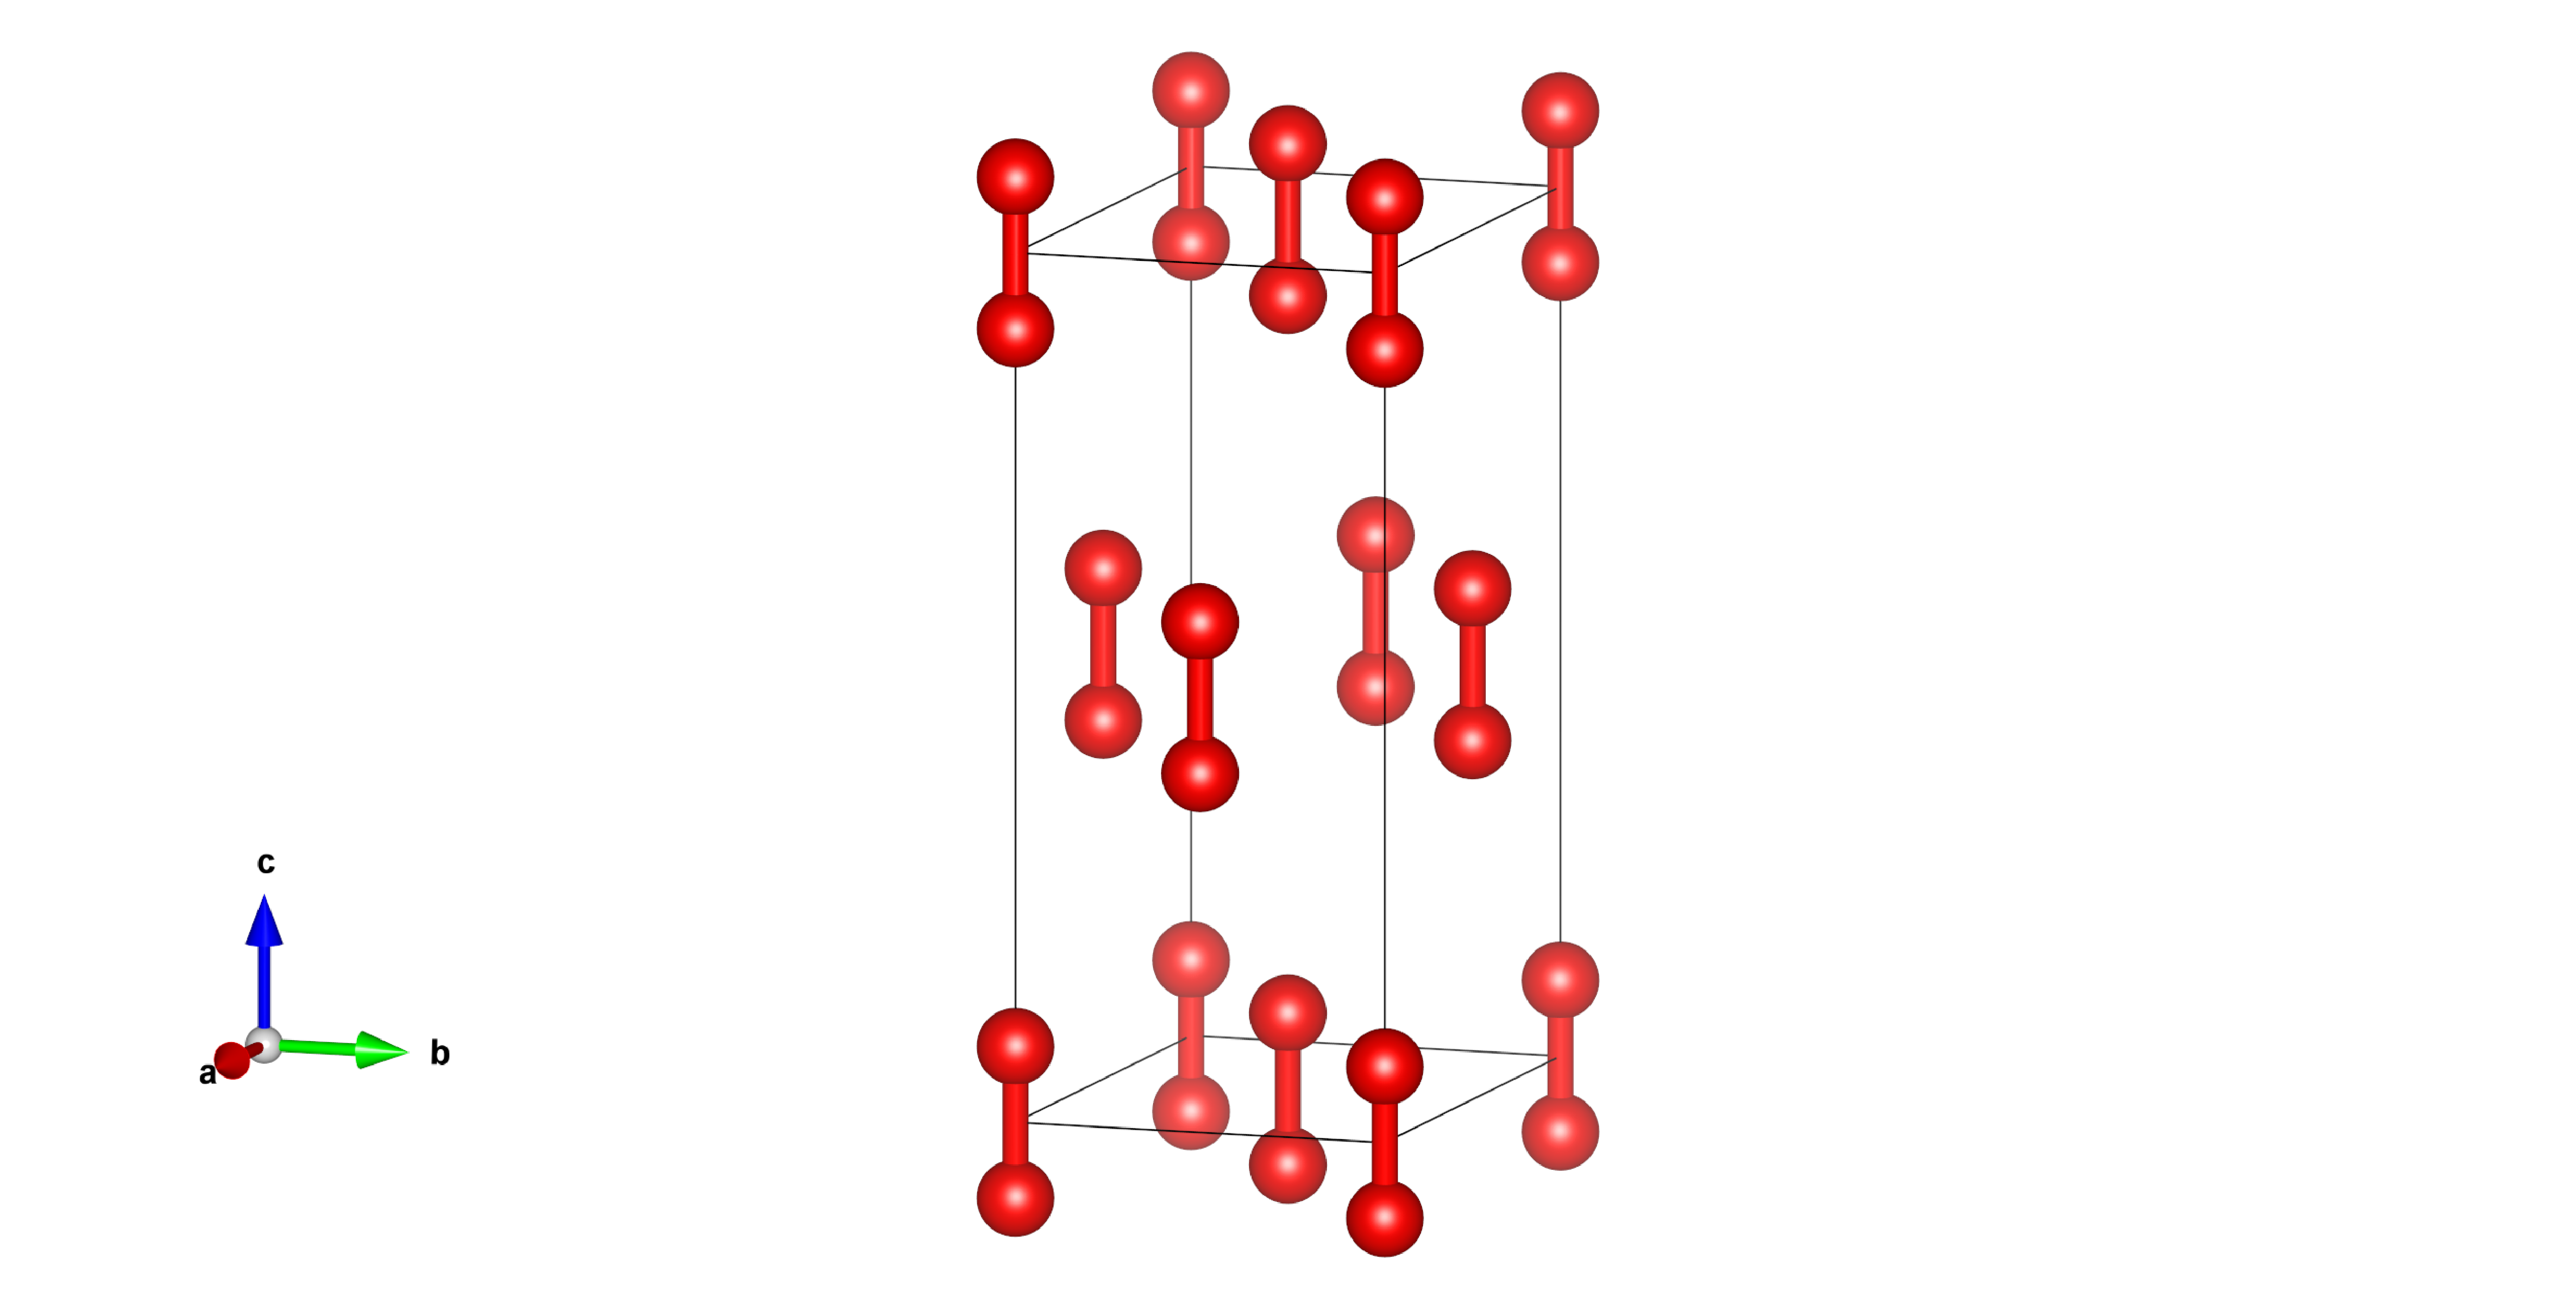
\includegraphics[scale=0.125]{picture/delta-O2.eps}
            \caption{$\delta$-$\ce{O2}$的晶体结构示意}
        \end{figure}
    \item $\ep$-$\ce{O2}$\\
        \indent 深红色至黑色晶体,属于单斜晶系,室温时生成于$9\text{ GPa}$以上.$\ep$-$\ce{O2}$又被称作\tbf{红氧},其中含有\ce{O2}的四聚体\ce{O8}.
        \begin{figure}[H]
            \centering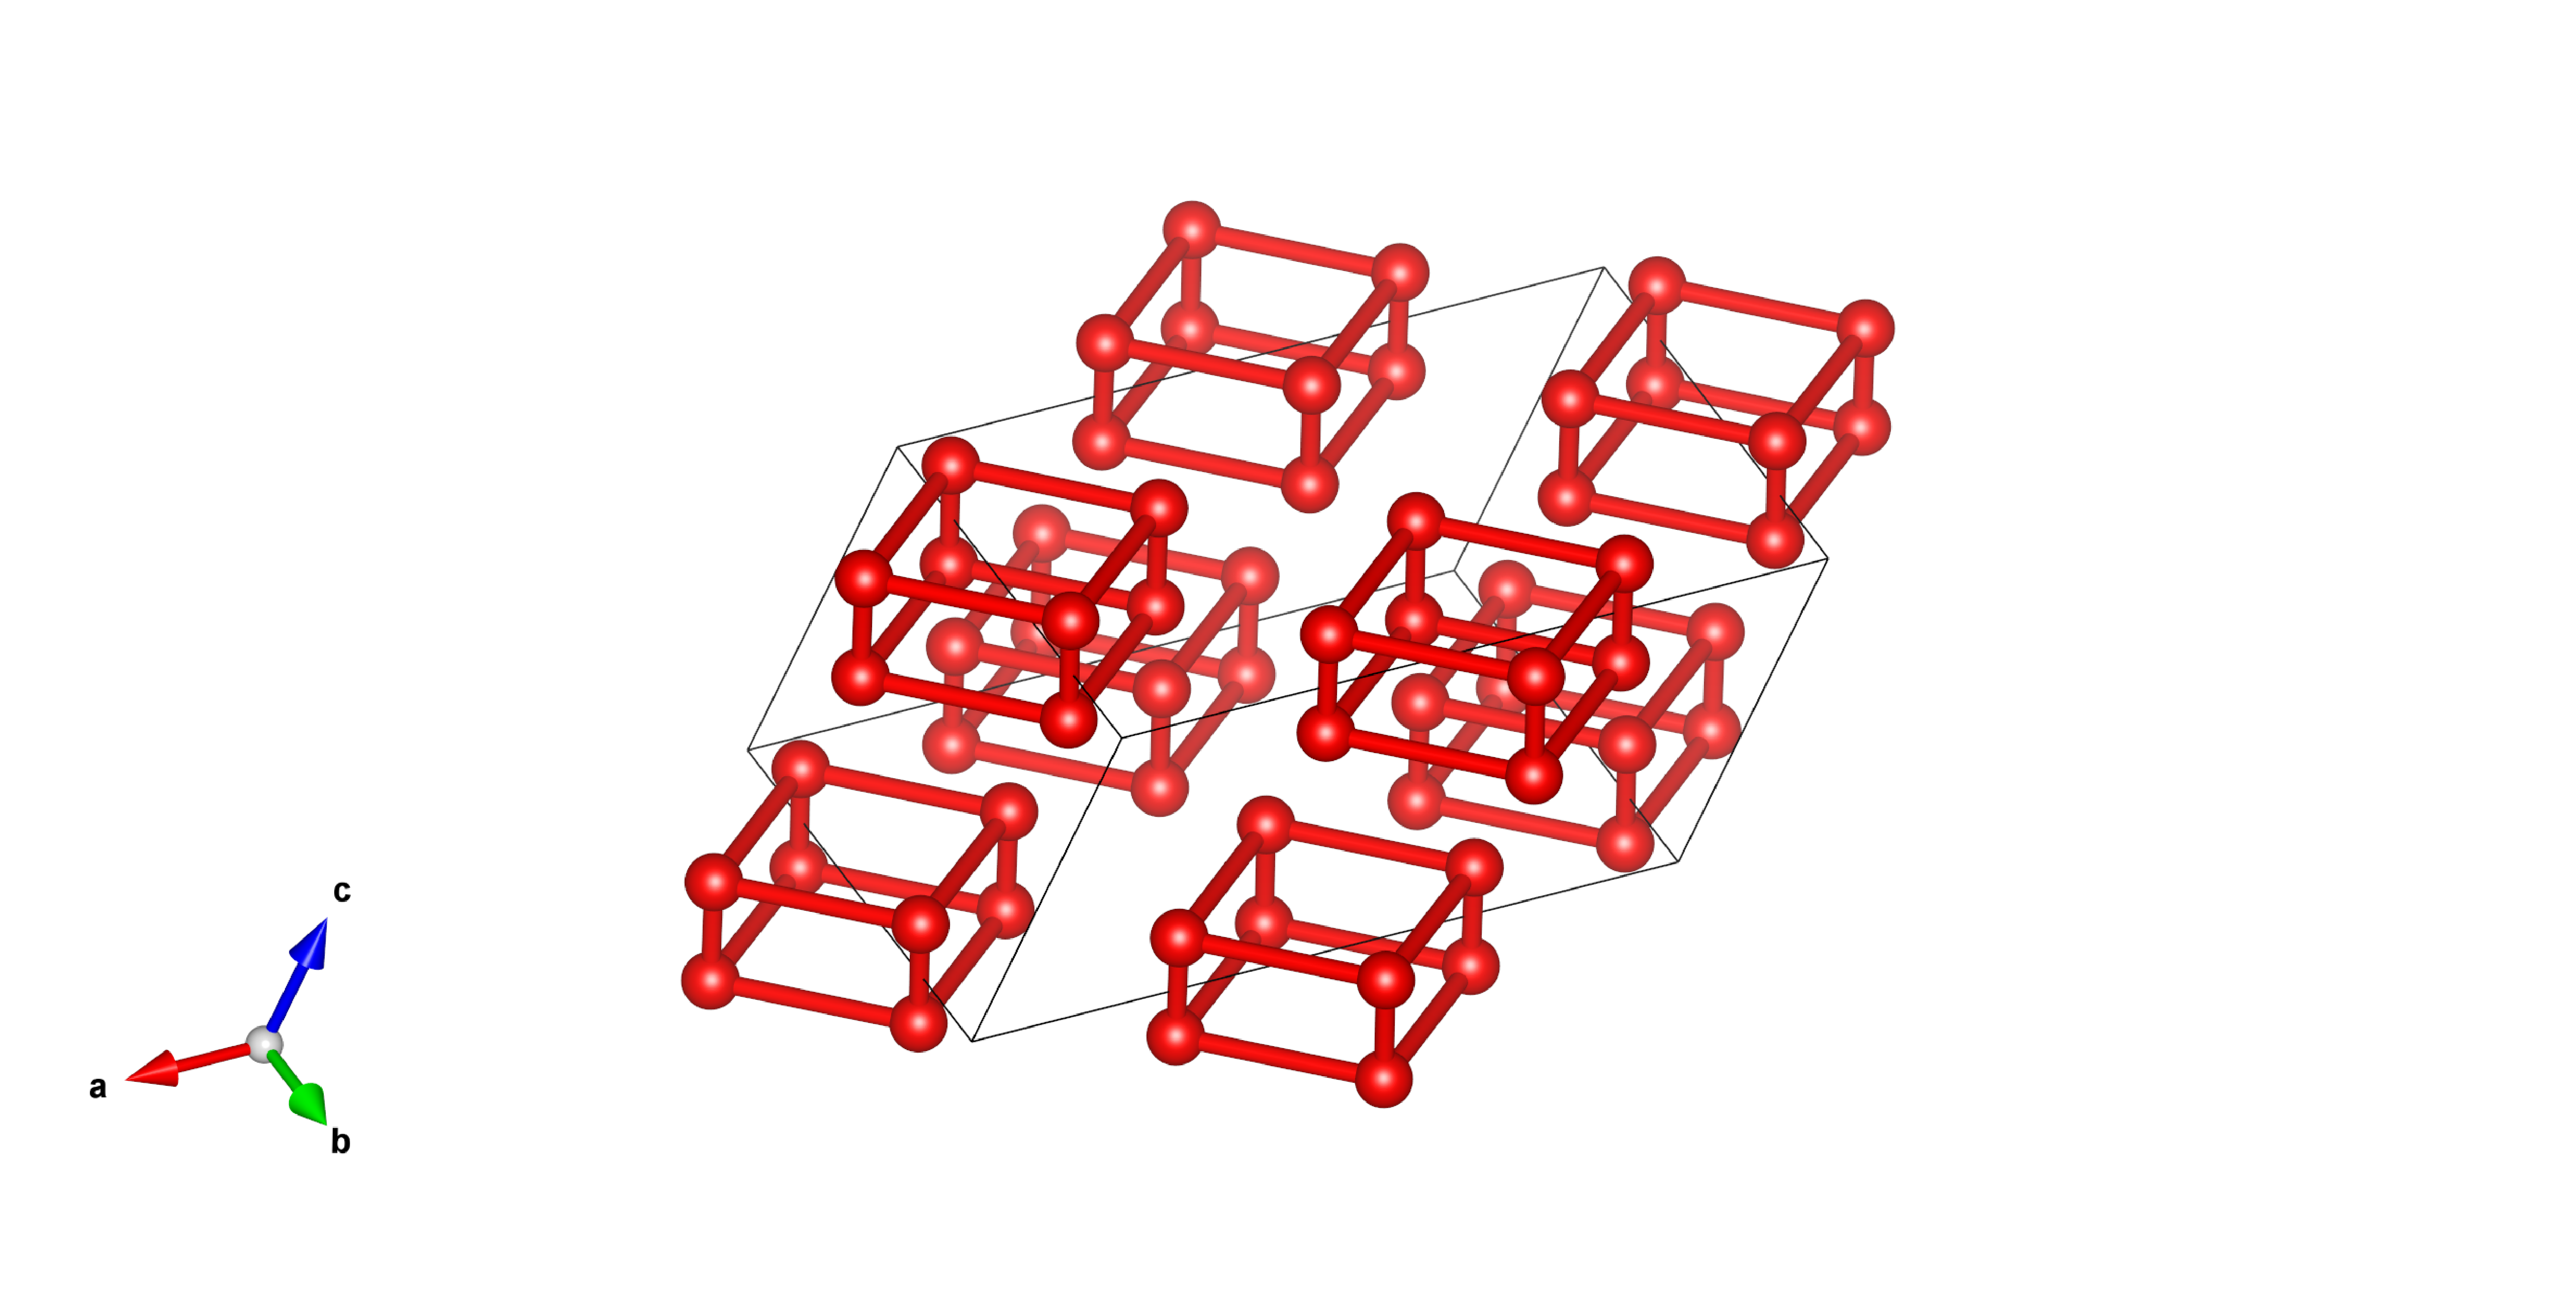
\includegraphics[scale=0.125]{picture/ep-O2.eps}
            \caption{$\ep$-$\ce{O2}$的晶体结构示意}
        \end{figure}
        可以看到,\ce{O8}是由四个\ce{O2}作用形成的菱面体簇合分子,这与\ce{S8}有明显区别.
\end{enumerate}
\subsubsection{\ce{O3}}
\begin{substance}[\ce{O3}]
    \ce{O3}俗称臭氧,室温下为淡蓝色气体,有淡淡的鱼腥味.常压下在$161.2\K$时液化为深蓝色液体,在$80.6\K$时凝固为紫黑色固体\footnotemark.
\end{substance}\footnotetext{值得注意的是,\ce{O3}和\ce{I2}是唯二的紫黑色固体单质.}
\paragraph{\ce{O3}的结构}
\ce{O3}为折线形分子,中心\ce{O}原子为sp$^2$杂化,键角为$116.8^\circ$.\ce{O3}的HOMO轨道系数最大处在两端的\ce{O}原子上,这与其共振式中两端\ce{O}原子带形式负电荷也相符合.
\begin{figure}[H]
    \centering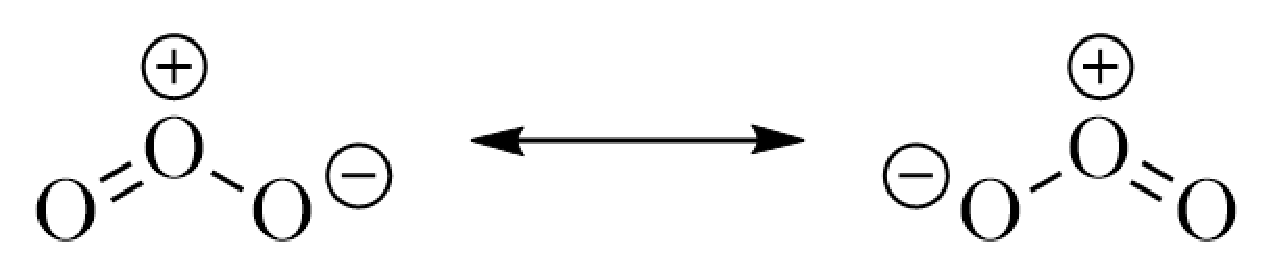
\includegraphics[scale=0.25]{picture/O3.eps}
    \caption{\ce{O3}的共振式}
\end{figure}
\paragraph{自然界中的\ce{O3}}自然界中的\ce{O3}主要来源于以下途径:
\begin{center}
    \ce{O2 ->T[$h\nu$][uv] 2O}\\
    \ce{O + O2 -> O3}
\end{center}
即\ce{O2}在光照作用下分解生成\ce{O}原子,\ce{O}原子再与\ce{O2}化合形成\ce{O3}.\\
\indent 除了\ce{O3}在光谱的红端$500\sim700\text{ nm}$处的强烈吸收使其显现蓝色以外,我们关心得更多的,\ce{O3}的另一个重要吸收区域位于紫外$220\sim290\text{ nm}$处,\ce{O3}吸收这一波长的光后重新分解形成\ce{O2}:
\begin{center}
    \ce{2O3 ->T[uv] 3O2}
\end{center}
大气中的臭氧层正是因此而将太阳辐射中的紫外线吸收,保护了地球表面居民们免遭强烈辐射.\\
\indent 然而,以氟利昂\ce{CClF3}为代表的物质对臭氧层有巨大破坏.它们性质稳定,进入大气后则被紫外光照射而生成\ce{Cl.}:
\begin{center}
    \ce{CClF3 ->T[$h\nu$] F3C. + Cl.}
\end{center}
而\ce{Cl.}可以催化\ce{O3}的分解:
\begin{center}
    \ce{O3 ->T[$h\nu$] O2 + O}\\
    \ce{Cl. + O3 -> O2 + ClO.}\\
    \ce{ClO. + O -> Cl. + O2}
\end{center}
\paragraph{\ce{O3}的反应}
\ce{O3}具有强氧化性,其标准电极电势数据如下:
\begin{center}
    \ce{O3 + 2H^+ + 2e^- -> O2 + 2H2O}\ \ \ $\varphi^\ominus=+2.076\text{ V}$\\
    \ce{O3 + H2O + 2e^- -> O2 + 2OH^-}\ \ \ $\varphi^\ominus=+1.24\text{ V}$
\end{center}
需要注意的是,\ce{O3}作为氧化剂,还原产物一般为\ce{O2}.\\
\indent 测定\ce{O3/O2}混合气体中\ce{O3}的含量可以通过碘量法.在硼酸缓冲液中,\ce{O3}与\ce{I^-}发生如下反应
\begin{center}
    \ce{O3 + 3I^- + 2H2O -> O2 + I3^- + 2OH^-}
\end{center}
然后用\ce{Na2S2O3}进行反滴定即可.注意氧化产物为\ce{I3^-},而没有进一步被氧化.这可能是动力学因素导致的.\\
\indent \ce{O3}作为氧化剂的其它典型反应列举如下:
\begin{center}
    \ce{O3 + CN^- -> OCN^- + O2}\\
    \ce{4O3 + PbS -> PbSO4 + 4O2}\\
    \ce{O3(g) + XeO3(aq) + 2H2O(l) -> H4XeO6(aq) + O2(g)}
\end{center}
等等.\\
\indent 关于\ce{O3}的另一类重要反应,即形成臭氧化物\ce{MO3}的反应,我们留到后面再叙.
\subsection{氧的化合物}
\subsubsection{$\mbf{-2}$氧化态:水}
\begin{substance}[\ce{H2O}]
    水的化学式为\ce{H2O},在常温下是无色无味的液体.在标准大气压下,水的沸点是$373.15\K$,凝固点是$273.15\K$.
\end{substance}
\paragraph{滴定微量\ce{H2O}的方法}
我们先来介绍测定微量水的方法—Karl Fischer法.这一方法的原理是\ce{I2}氧化\ce{SO2}时需要定量的水参与反应:
\begin{center}
    \ce{I2 + SO2 + 2H2O -> 2HI + H2SO4}
\end{center}
然而,实际条件下需要加入碱使得反应进行得完全.一般选用吡啶和甲醇作为辅助试剂,此时\ce{I2}与\ce{H2O}的计量比为$1:1$,反应方程式为
\begin{center}
    \ce{3py + SO2 + I2 + H2O + MeOH -> 2[pyH]^+I^- + [pyH]^+[MeOSO3]^-}
\end{center}
滴定时,将试样加入甲醇溶液中,然后用含有\ce{I2},\ce{SO2}和吡啶的甲醇溶液(即Fischer试剂)进行滴定.过量的Fischer试剂显示棕色,可以作为判断终点的依据.\\
\indent 需要注意的是,这一方法的计量比很容易被混淆\footnote{Fischer当年发明这一方法时就弄错了计量比,直到后来才被纠正.}.\paragraph{水的电离与水合质子}我们已经知道水可以进行自耦电离:
\begin{center}
    \ce{2H2O(l) <=> H3O^+(aq) + OH^-(aq)}\ \ \ $K_\text{h}=1.0\times10^{-14}$
\end{center}
\indent 除了\ce{H3O^+}以外,还有多种多样的水合质子\ce{H_{2n+1}O_n^+}.它们的结构如下.
\begin{enumerate}[label=\tbf{\arabic*},topsep=0pt,parsep=0pt,itemsep=0pt,partopsep=0pt]
    \item \ce{H3O^+}.作为\ce{NH3}的等电子体,\ce{H3O^+}也是三角锥型的离子.它存在于\ce{[H3O][SbF6]},\ce{[H3O][HSO4]}等多种晶体中.
        \begin{figure}[H]
            \centering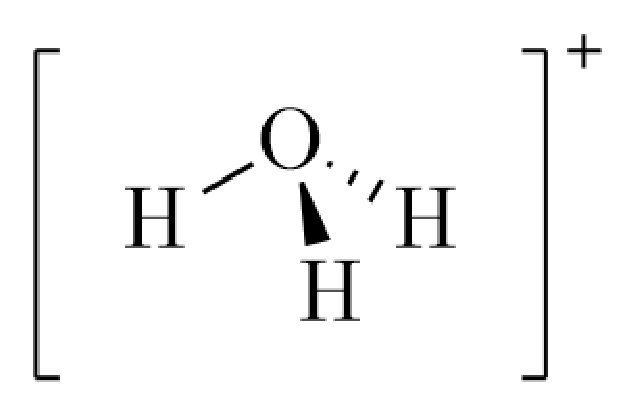
\includegraphics[scale=0.25]{picture/H3O+.eps}
            \caption{\ce{H3O+}的结构}
        \end{figure}
    \item \ce{H5O2+}.它存在于多种晶体中,既有交错式,也有重叠式.
        \begin{figure}[H]
            \centering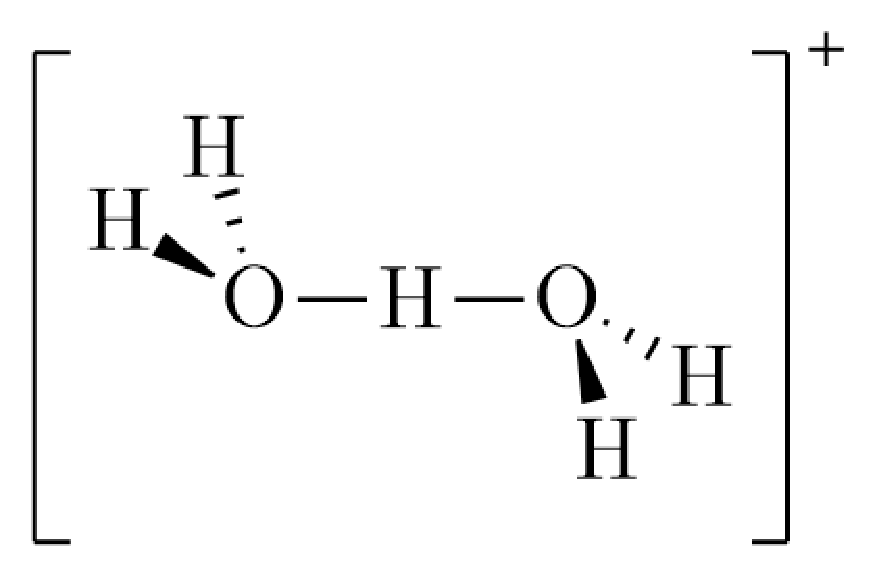
\includegraphics[scale=0.25]{picture/H5O2+.eps}
            \caption{\ce{H5O2+}的结构}
        \end{figure}
    \item \ce{H7O3+}和\ce{H9O4+}.
        \begin{figure}[H]
            \centering
            \subfigure[\ce{H7O3+}]
            {
                \begin{minipage}[b]{.45\linewidth}
                    \centering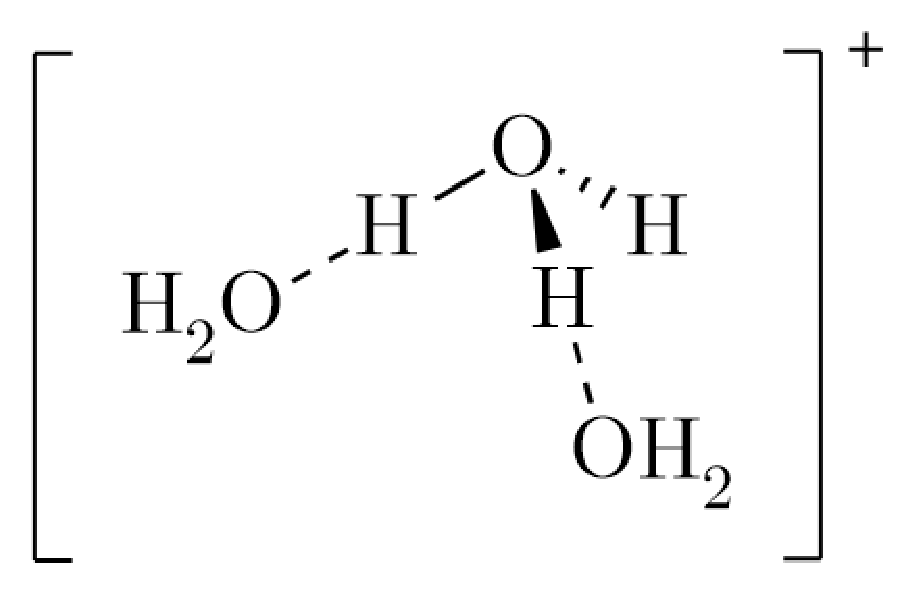
\includegraphics[scale=0.25]{picture/H7O3+.eps}
                \end{minipage}
            }
            \subfigure[\ce{H9O4+}]
            {
                \begin{minipage}[b]{.45\linewidth}
                    \centering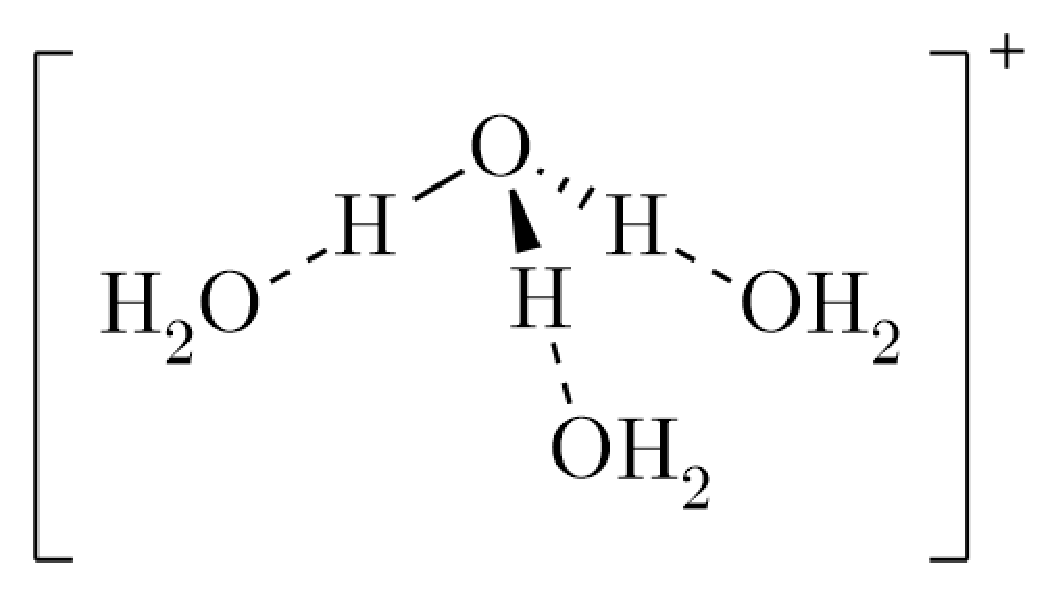
\includegraphics[scale=0.25]{picture/H9O4+.eps}
                \end{minipage}
            }
            \caption{\ce{H7O3+}和\ce{H9O4+}的结构}
        \end{figure}
    \item \ce{H13O6+}.它最初被发现于笼状阳离子\ce{[(C9H18)3(NH)2Cl]^+}在盐酸溶液析出的结晶中.该固体中的\ce{H13O6+}被周围的\ce{Cl-}离子所稳定.下面是该笼状阳离子结构和水合氢离子的结构.
        \begin{figure}[H]
            \centering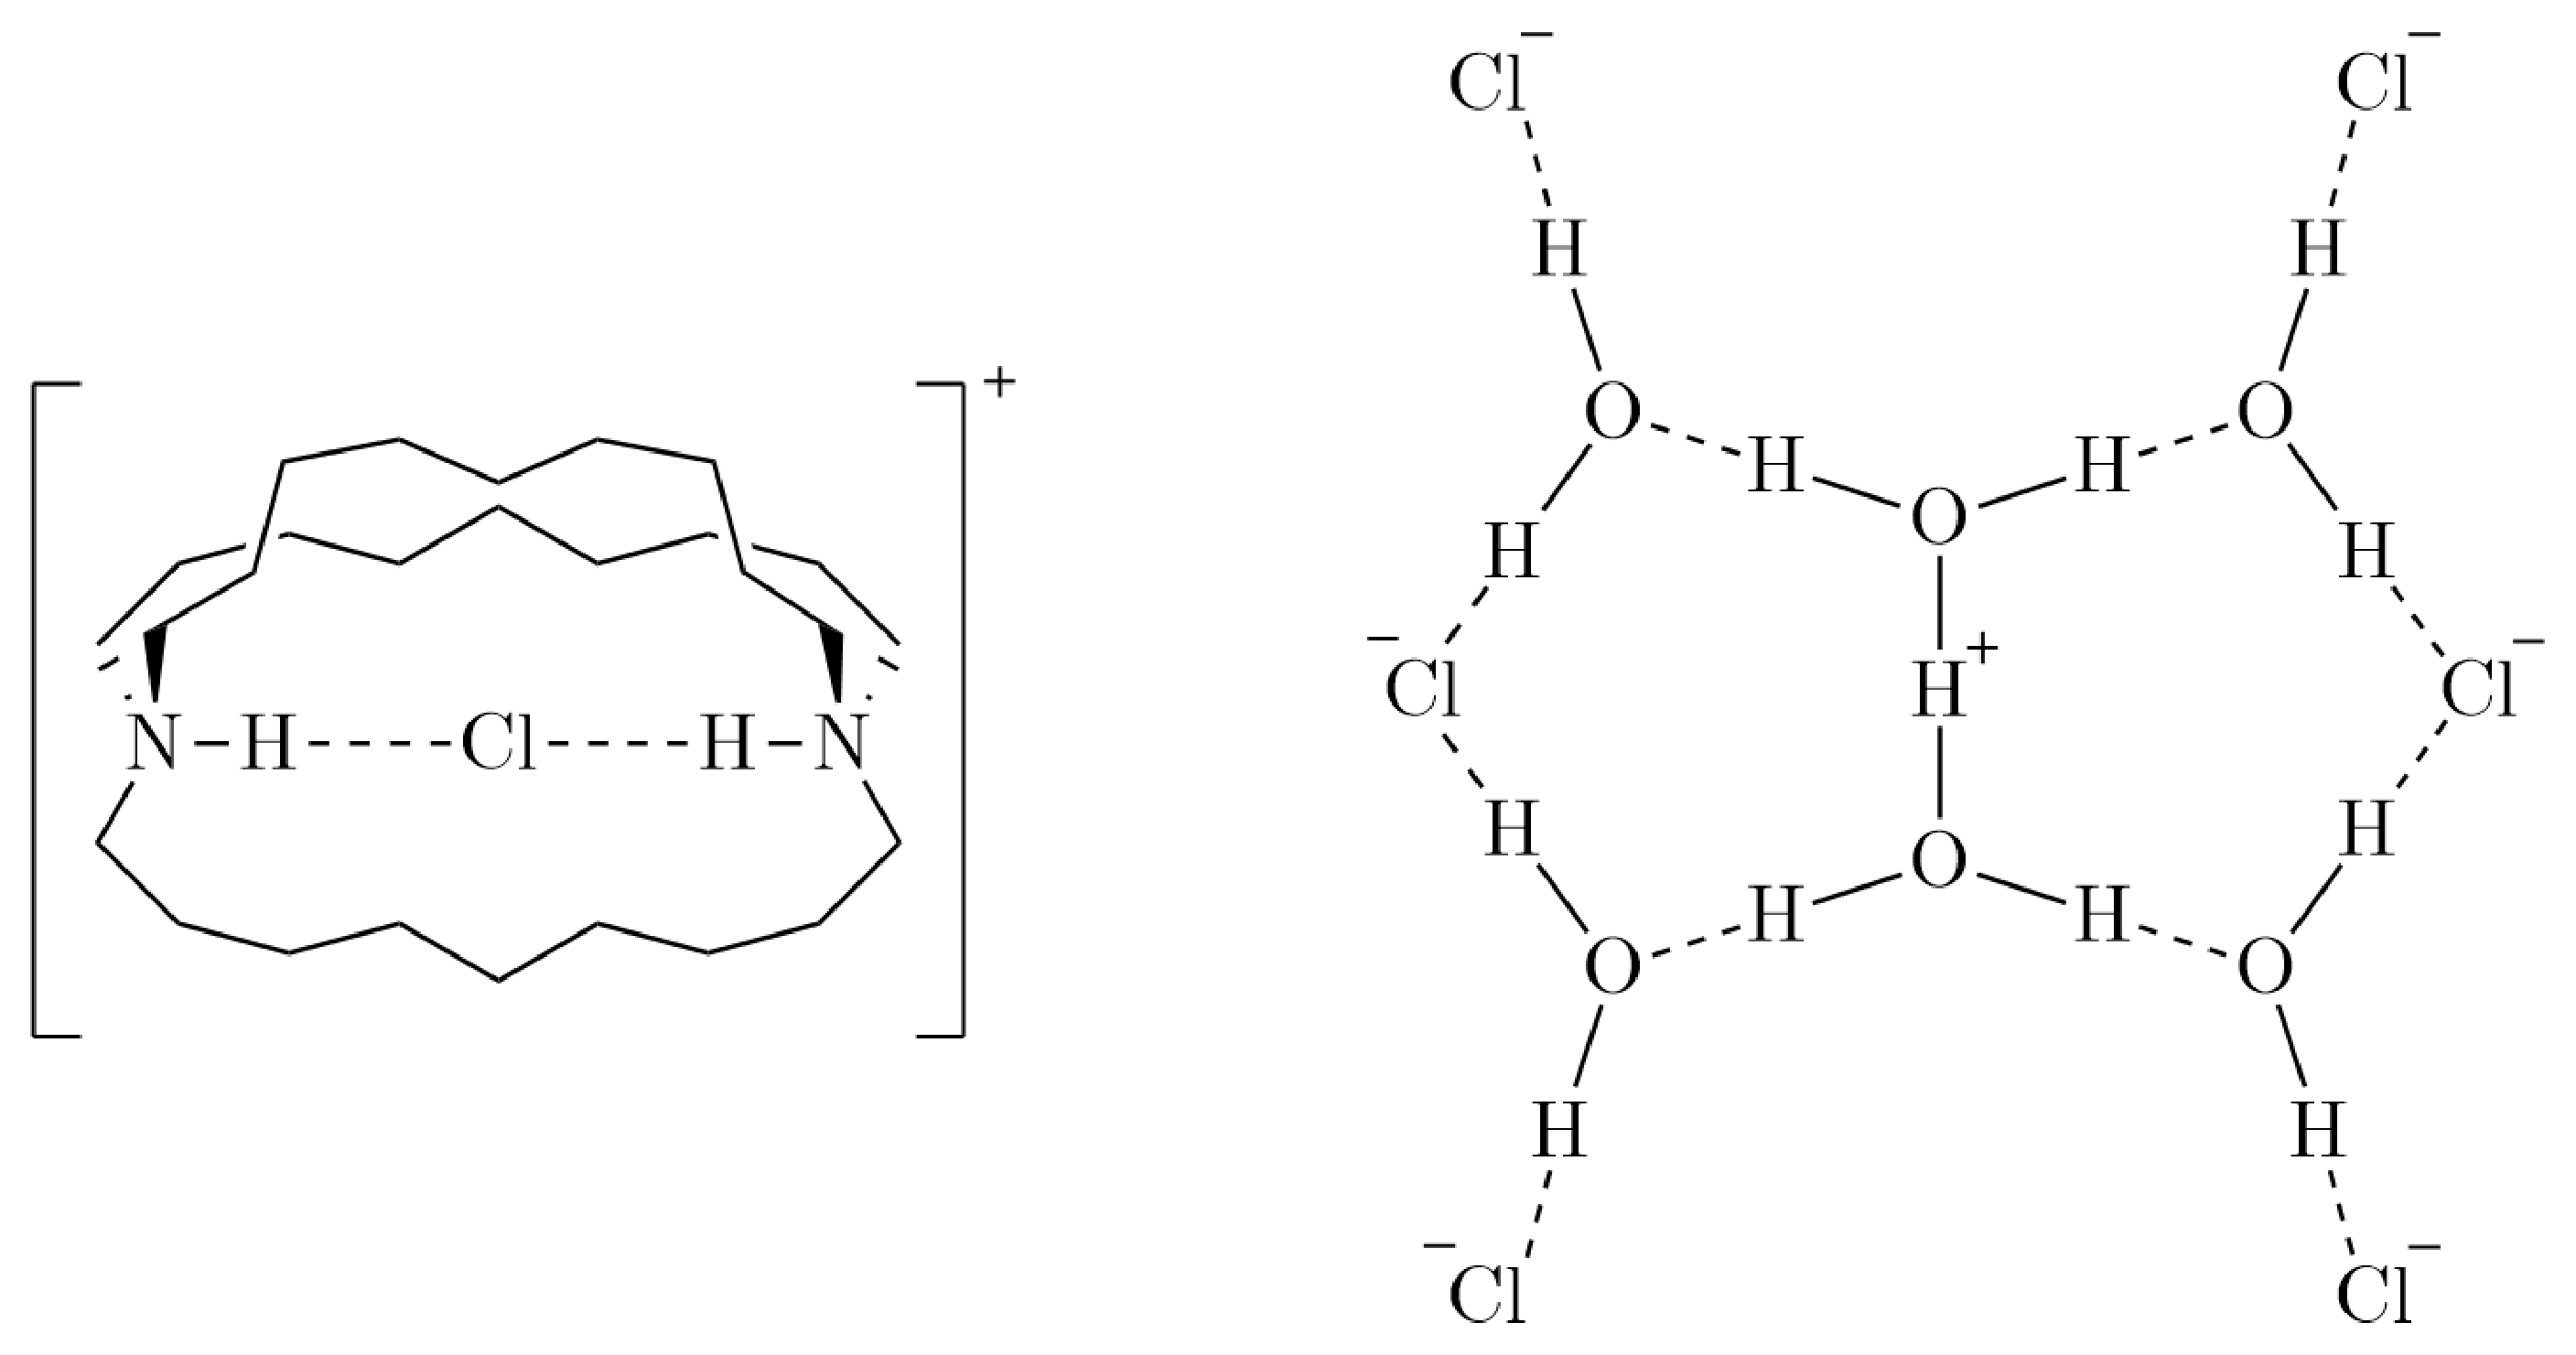
\includegraphics[scale=0.25]{picture/H13O6+.eps}
            \caption{\ce{[(C9H18)3(NH)2Cl]^+}和\ce{H13O6+}的结构}
        \end{figure}
\end{enumerate}
\paragraph{各种晶型的冰}我们现在来介绍各种晶型的冰.
\begin{enumerate}[label=\tbf{\arabic*},topsep=0pt,parsep=0pt,itemsep=0pt,partopsep=0pt]
    \item 冰-$I_h$\\
        冰-$I_h$是冰的最常见的晶型,其晶体结构示意如下.
        \begin{figure}[H]
            \centering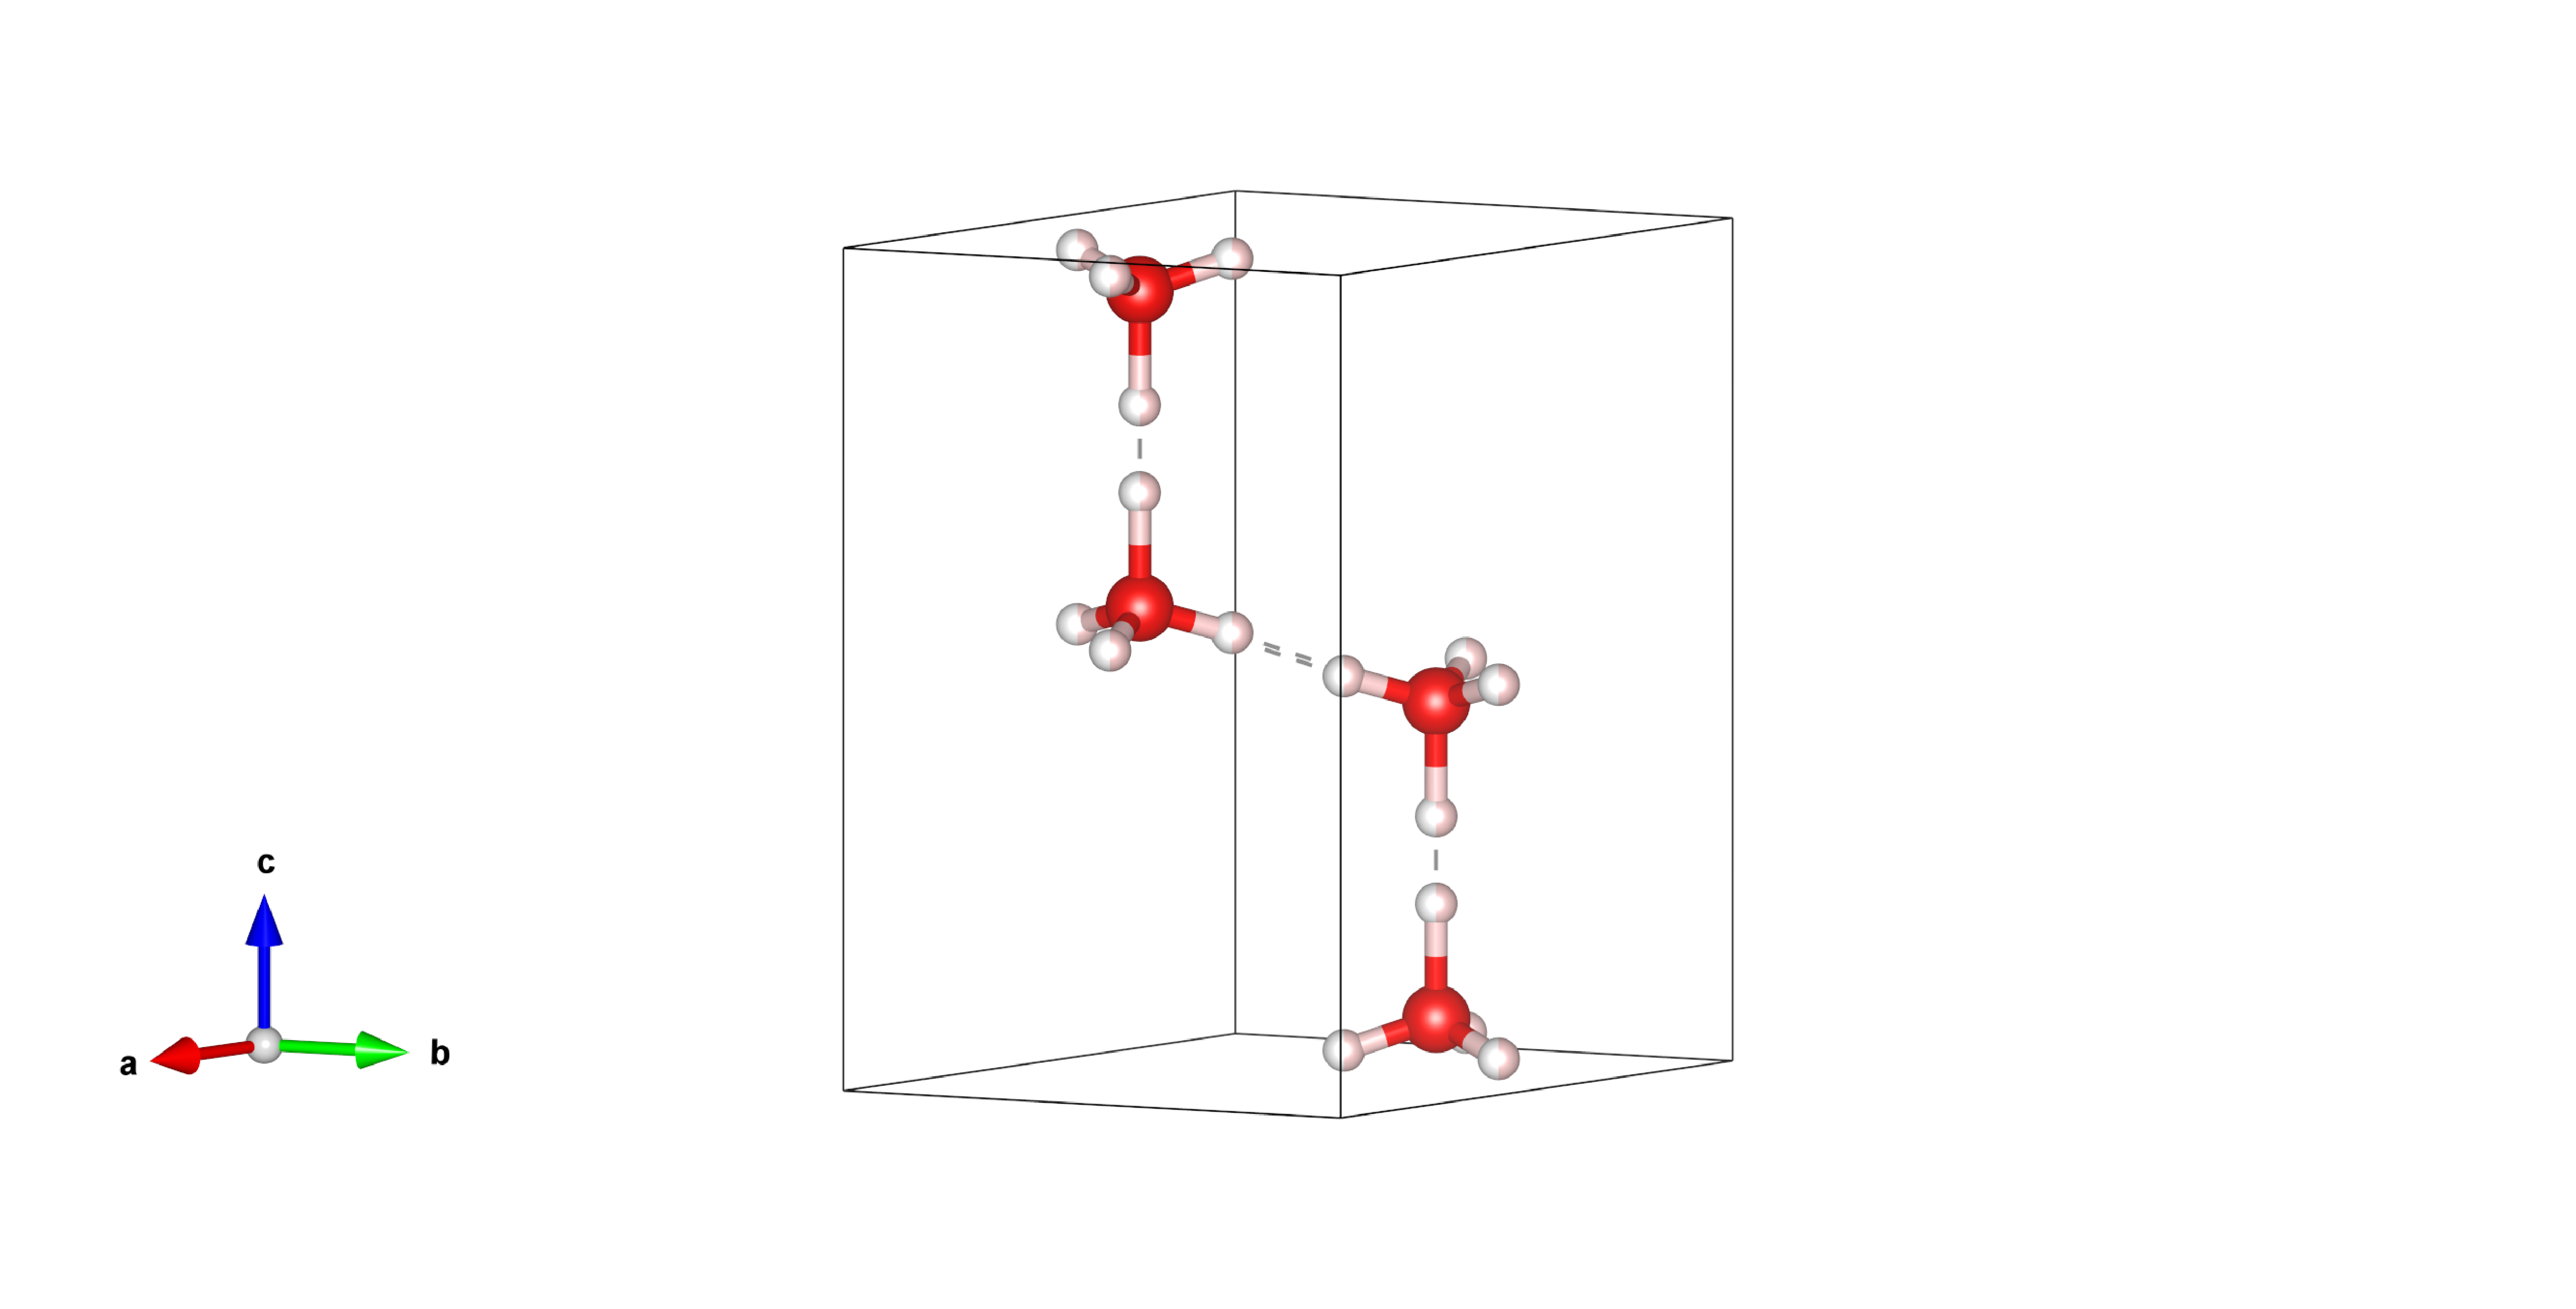
\includegraphics[scale=0.125]{picture/Ih-Ice.eps}
            \caption{冰-$I_h$的晶体结构}
        \end{figure}
        冰-$I_h$中,\ce{O}做六方密堆积,每两个\ce{O}之间有一个\ce{H}原子.所有\ce{H}都是统计分布的,它与某一边的\ce{O}形成化学键,与另一边的\ce{O}形成氢键.\\
        一个值得考虑的问题是冰-$I_h$的残余熵.我们可以推导如下.
        \begin{derivation}
            考虑到六方冰中O原子做六方密堆积排列,因此O的位置就固定不动.\\
            由于固态的冰中存在氢键网络,每个O原子都通过氢键和周围四个O原子连接,因此我们需要做一个假设,%
            即每个O原子周围都有两个H与其距离较远,另外两个与其距离较近.这对应着O形成两根O$-$H化学键和两根O$\cdot\cdot$H氢键.\\
            这样,我们只需要考虑H的位置即可.对于1\ mol冰中的2\ mol\ H原子,都有两种状态,即处于两个O原子之间离其中某个O原子更近的位置.%
            这样的微观状态数一共有$2^{2\NA}$种.\\
            考虑到O原子对H原子的位置,每个O原子周围恰好有两个H靠近,两个H远离.这样的概率为
            \[P_O=\dfrac{C_4^2}{2^4}=\dfrac{3}{8}\]
            于是总的微观状态数为
            \[\Omega=2^{2\NA}\cdot\left(P_O\right)^{\NA}=\left(\dfrac32\right)^{\NA}\]
            于是
            \[S=k_\text B\ln\Omega=R\ln\dfrac32\JmK\approx3.37\JmK\]
            
        \end{derivation}
        冰-$I_h$的氢键网络使得其密度小于水.当冰-$I_h$融化时,约有$\dfrac14$的氢键被破坏,并且这一比例将随着温度升高而持续增大,从而使得\ce{H2O}分子相互靠近,密度增大.另一方面,温度升高将使得分子热运动加剧,从而使密度减小.这两个效应的净结果是\ce{H2O}的密度在$3.98\tccentigrade$时达到最大.
    \item 冰-$I_c$\\
        冰-$I_c$的结构与冰-$I_h$十分相近,区别只在于冰-$I_c$中的\ce{O}原子做立方最密堆积,而\ce{H}分布的方式则相同.
\end{enumerate}
\subsubsection{$\mbf{-1}$氧化态}
在\ce{O}的\ce{-1}氧化态中最重要的化合物就是过氧化氢.%
其余的过氧化物,处于内容的连续性的考虑,放在\tbf{1.2.4}中进行介绍.
\begin{substance}[\ce{H2O2}]
    过氧化氢,化学式为\ce{H2O2}.纯净的\ce{H2O2}为几乎无色(带有非常浅的蓝色)的液体.\ce{H2O2}可以与\ce{H2O}任意比例地互溶,这是由于两者形成氢键的缘故.实验室中常用的是3\%$\sim$30\%的过氧化氢水溶液,称为双氧水.
\end{substance}
\paragraph{\ce{H2O2}的酸碱性}
\ce{H2O2}是比\ce{H2O}稍强的酸:
\begin{center}
    \ce{H2O2 + H2O <=> H3O^ + HOO^-}\ \ \ $K_\text a=1.78\times10^{-12}$
\end{center}
这可能是由于\ce{O}的吸电子效应所致.另一方面,\ce{HOO^-}是比\ce{HO^-}更好的亲核试剂,因为两个\ce{O}原子的孤对电子排斥使得HOMO能量升高.\\
\indent 也正因为\ce{O}的吸电子效应,\ce{H2O2}的碱性比\ce{H2O}弱得多.下面这一反应
\begin{center}
    \ce{H3O2^+ + H2O -> H3O^+ + H2O2}
\end{center}
的平衡常数估计在$10^6$以上.\\
\indent 液氨能与\ce{H2O2}反应生成白色的\ce{NH4OOH}固体,其中含有\ce{NH4+}和\ce{OOH-}离子,但熔融时似乎只存在由氢键联系的\ce{NH3}和\ce{H2O2}分子.这导致其熔点只有$25\tccentigrade$,明显低于一般的离子化合物.
\paragraph{\ce{H2O2}的氧化还原性}在酸性条件下,\ce{H2O2}是很好的氧化剂,但在强氧化剂存在时也可以作为还原剂.
\begin{center}
    $\varphi^\ominus_{\text{Acid}}$:\ \ \ \ce{O2 ->T[$0.68\text{ V}$] H2O2 ->T[$1.77\text{ V}$] H2O}
\end{center}

\indent 而在碱性条件下,\ce{H2O2}是中等的氧化剂.
\begin{center}
    $\varphi^\ominus_{\text{Base}}$:\ \ \ \ce{O2 ->T[$-0.076\text{ V}$] HO2^- ->T[$0.878\text{ V}$] H2O}
\end{center}

\indent 无论是作为氧化剂还是还原剂,\ce{H2O2}在水溶液体系中都不会引入杂质.因此,\ce{H2O2}是实验室中常用的氧化剂.\\
\indent 从标准电极电势看,\ce{H2O2}容易发生歧化.这在由催化剂的存在下进行地十分迅速.事实上,这一分解反应的催化剂大多是那些处于氧化态时可以氧化\ce{H2O2},处于还原态时可以被\ce{H2O2}氧化的物质.我们以$\ce{Fe^3+}/\ce{Fe^2+}$电对为例,催化反应的方程式为
\begin{center}
    \ce{2Fe^2+ + H2O2 + 2H+ -> 2Fe^3+ + 2H2O}\\
    \ce{2Fe^3+ + H2O2 -> 2Fe^2+ + O2 + 2H^+}\\
    总反应:\ce{2H2O2 ->T[\ce{Fe^3+}][\ce{Fe^2+}] 2H2O + O2}
\end{center}
因此,在酸性溶液中还原电势处于$0.68\text{ V}$和$1.77\text{ V}$之间的物质理论上均可催化这一反应.各种过渡金属离子,例如\ce{Fe^2+},\\\ce{Mn^2+},\ce{Cr^3+}的存在都会加速这一反应.此外,光照或加热也可以促使\ce{H2O2}分解.因此需要将其存放在棕色瓶中在避光阴凉处保存,并加入稳定剂(常用的有\ce{Na2SnO3},\ce{Na4P2O7}和8-羟基喹啉等).
\paragraph{\ce{H2O2}的制备} J.L.Thenard于1818年首次通过酸化\ce{BaO2}的方式后减压蒸除\ce{H2O}的方式制得了\ce{H2O2}.
\begin{center}
    \ce{BaO2 + H2SO4 -> BaSO4 + H2O2}
\end{center}

\indent 后来,人们采用电解-水解法制备\ce{H2O2}.
\begin{center}
    \ce{2NH4HSO4 ->T[电解] (NH4)2S2O8 + H2}\\
    \ce{(NH4)2S2O8 + 2H2O -> 2NH4HSO4 + H2O2}
\end{center}

\indent 但以上两种方法都已被乙基蒽醌法所取代.这一方法采用乙基蒽醌和\ce{Pd}作为催化剂,由\ce{H2}和\ce{O2}直接合成\ce{H2O2},具体反应过程如下.
\begin{figure}[H]
    \centering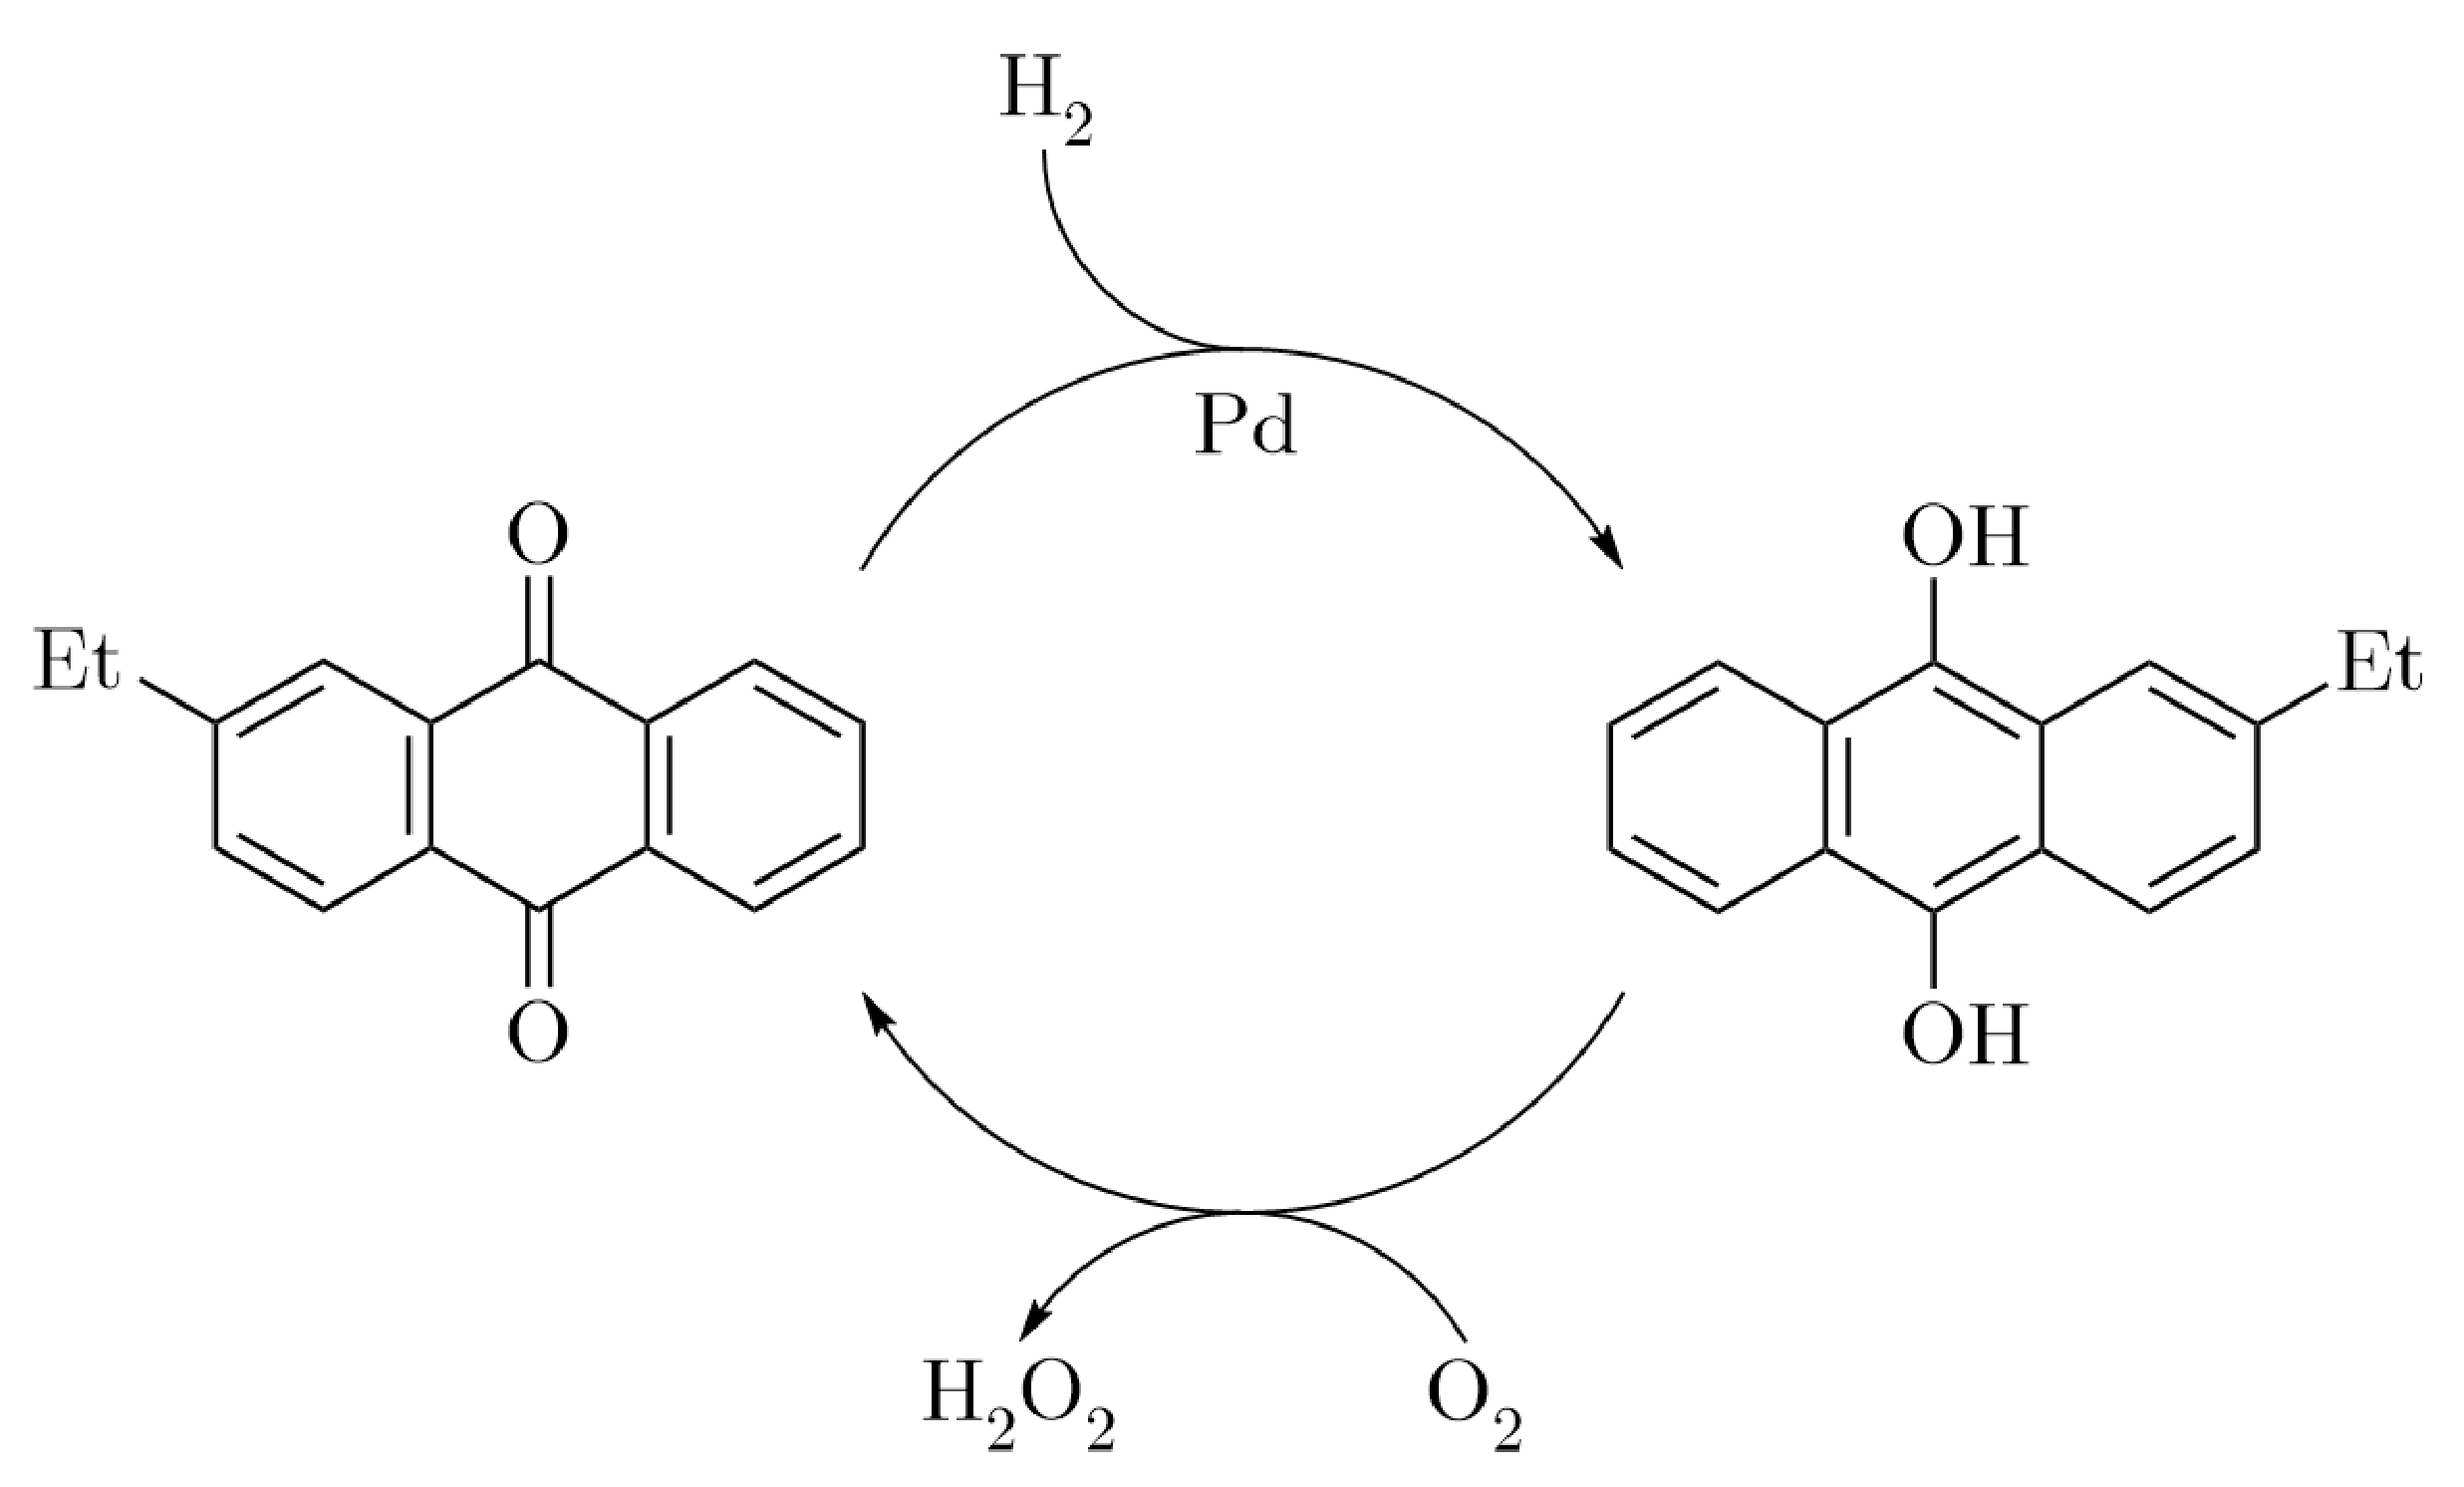
\includegraphics[scale=0.25]{picture/H2O2Prod.eps}
    \caption{乙基蒽醌法制备\ce{H2O2}}
\end{figure}
工业上采取此方法大量地合成\ce{H2O2}.
\subsubsection{正氧化态:氧的氟化物}
由于氧的高电负性,几乎只有在与氟形成共价键时才显正价.典型的物质有\ce{OF2},\ce{HOF}和\ce{O2F2}等.
\begin{substance}[\ce{OF2}]
    \ce{OF2}是一种无色,剧毒的气体,可以冷凝为淡黄色的液体.纯净的\ce{OF2}对热稳定,直到$200\tccentigrade$才开始分解.
\end{substance}
\begin{substance}[\ce{HOF}]
    \ce{HOF}是一种白色固体,于$-117\tccentigrade$熔化为淡黄色液体.\ce{HOF}在室温下迅速地分解为\ce{HF}和\ce{O2}.
\end{substance}
\begin{substance}[\ce{O2F2}]
    \ce{OF2}是一种黄色固体,于$-154\tccentigrade$熔化为淡黄色液体.\ce{O2F2}极不稳定,甚至在$-160\tccentigrade$就以每日约$4\%$的速度分解.
\end{substance}
\paragraph{氧的氟化物的结构} 不出所料地,\ce{OF2}和\ce{HOF}均为折线形分子.它们的键角数据如下(作为对比,这里一并放上\ce{H2O}的键角数据):
\begin{center}
    \ce{OF2}\ \ \ $\angle\left(\ce{F-O-F}\right)=103^\circ$\\
    \ce{HOF}\ \ \ $\angle\left(\ce{H-O-F}\right)=97^\circ$\\
    \ce{H2O}\ \ \ $\angle\left(\ce{H-O-H}\right)=104.5^\circ$
\end{center}

\indent \ce{HOF}的键角明显比另外两者更小\footnote{一种扯淡的解释是\ce{H}和\ce{F}之间的经典吸引作用.}.%
这一点可以用\tbf{配体紧密堆积模型}\footnote{R.J. Gillespie, Coord. Chem. Rev. 197 (2000) 51, https://doi.org/10.1016/S0010-8545(99)00199-X,}(LCP模型)进行解释.%
LCP模型认为具有两个或多个不同配体的分子中,配位原子间距等于或接近相应配体半径之和.对于\ce{HOF}而言,\ce{H-O}键明显短于\ce{F-O}键,这意味着键角需要更小以满足\ce{H}与\ce{F}之间距离为配体半径之和的条件\footnote{关于LCP模型的更多应用,应该会在后面再提到.}.\\
\indent \ce{O2F2}和\ce{H2O2}的结构相似.值得注意的是,\ce{O2F2}中的\ce{O-O}键长为$121.7\text{ pm}$,明显小于\ce{H2O2}中的$147.5\text{ pm}$;而\ce{O2F2}中的\ce{O-F}键长为$157.5\text{ pm}$,明显大于\ce{OF2}中的$140.5\text{ pm}$.这可能是由于氧原子的孤对电子对$\sigma^\ast\left(\ce{O-F}\right)$轨道的超共轭效应削弱\ce{O-F}键而增强\ce{O-O}键所致.
\paragraph{氧的氟化物的合成} \ce{OF2}是上述三种化合物中最稳定的,其制备方式也比较简单,将\ce{F2}通入\ce{NaOH}溶液即可:
\begin{center}
    \ce{2F2 + 2NaOH -> 2NaF + OF2 + H2O}
\end{center}

\indent 没有证据表明\ce{OF2}能与水反应生成\ce{HOF},因此\ce{OF2}严格意义上不能称作次氟酸酐.\ce{HOF}需要于低温下\ce{F2}与\ce{H2O}反应得到(最初是在\ce{N2}气氛中将\ce{F2}缓慢通过碎冰的表面而少量得到的):
\begin{center}
    \ce{H2O + F2 -> HF + HOF}
\end{center}
\indent 而\ce{O2F2}则需要通过对\ce{O2}和\ce{F2}的混合气体低压放电得到.
\paragraph{\ce{HOF}的反应}
HOF具有强烈的氧化性.典型的反应如下.
\begin{center}
    \ce{BrO3- + HOF -> BrO4- + HF}
\end{center}
鉴于\ce{F2}能氧化\ce{BrO3-}为\ce{BrO4-},这很可能就是反应体系中发生的主要反应之一.
\subsubsection{复杂价态的含氧阴离子}
\paragraph{过氧化物}
我们主要讨论碱金属的过氧化物.它们都可以视作\ce{H2O2}的盐,其中含有过氧根阴离子\ce{O2^2-}.除了\ce{Li2O2}以外,其它碱金属的过氧化物都有着较好的热稳定性.
\begin{substance}[\ce{Li2O2}]
    过氧化锂,化学式为\ce{Li2O2},外观为白色晶型固体.\ce{Li2O2}的热稳定性尚可,在$195\tccentigrade$以上开始分解为\ce{Li2O}.
\end{substance}
工业上制备\ce{Li2O2}是让\ce{LiOH}与\ce{H2O2}反应后减压脱水而得.
\begin{substance}[\ce{Na2O2}]
    过氧化钠,化学式为\ce{Na2O2},外观为浅黄色粉末状固体.\ce{Na2O2}是\ce{Na}在过量\ce{O2}下燃烧的最终产物,直到约$675\tccentigrade$以上才开始分解.
\end{substance}
正如上面所说,直接对\ce{Na2O}氧化就可以制备\ce{Na2O2}.用这种方法制备\ce{K2O2},\ce{Rb2O2}和\ce{Cs2O2}则较为困难,因为它们很容易被继续氧化为超氧化物.\\
\indent 过氧化物在工业上作为漂白剂和强氧化剂使用.
\paragraph{超氧化物}
超氧化物\ce{MO2}含有顺磁性的超氧根阴离子\ce{O2^-}.%
只有较大的阳离子(\ce{K^+},\ce{Rb^+},\ce{Cs^+})形成的超氧化物才是较稳定的,对应的碱金属在足量空气中燃烧的产物即为超氧化物.而\ce{Na}和\ce{Li}的超氧化物则需要在低温条件下合成.这再一次说明了极化作用对离子化合物稳定性的影响.
\paragraph{臭氧化物}
臭氧化物\ce{MO3}中含有顺磁性的\ce{O3^-}.它们都是红棕色固体,其稳定性以$\ce{Cs}>\ce{Rb}>\ce{K}>\ce{Na}$的顺序降低,而尚且没有制备出\ce{LiO3}.\\
\indent 制备\ce{MO3}的最佳方法是将\ce{O3}与干燥的\ce{MOH}粉末作用,再用液氨萃取其中的\ce{MO3}.以\ce{KO3}为例,反应的方程式如下:
\begin{center}
    \ce{5O3 + 2KOH -> 2KO3 + 5O2 + H2O}
\end{center}
这一反应的计量系数比较古怪,是同位素标记所得出的结果.
\end{document}